%\documentclass[aspectratio=43]{beamer}
%\documentclass[aspectratio=169]{beamer}
\documentclass[aspectratio=1610,12pt]{beamer}
\usepackage[utf8]{inputenc}
\usepackage[T1]{fontenc}
\usepackage{lmodern}

\usepackage[ngerman]{babel}
%\usepackage[ngerman]{babel} %use this for German presentations
\usepackage{booktabs} % fancy tables
\usepackage{tabulary} % tables with auto column length
\usepackage{hyperref}
\newcommand{\enquote}[1]{{\glqq#1\grqq{}}}

\usepackage{tikz}
\usepackage{xcolor}
\usetikzlibrary{decorations.text}
\definecolor{mygray}{RGB}{208,208,208}
\definecolor{myred}{HTML}{FF0000}
\definecolor{mypink}{HTML}{FF8080}
\definecolor{mygreen}{HTML}{80FF80}
\newcommand*{\mytextstyle}{\sffamily\normalfont\bfseries\color{black!85}}
\newcommand{\arcarrow}[4]{%
   % inner radius, middle radius, outer radius, start angle,
   % end angle, tip protusion angle, options, text
   \pgfmathsetmacro{\rin}{2.5}
   \pgfmathsetmacro{\rmid}{3.0}
   \pgfmathsetmacro{\rout}{3.5}
   \pgfmathsetmacro{\astart}{#1}
   \pgfmathsetmacro{\aend}{#2}
   \pgfmathsetmacro{\atip}{5}
   \fill[#4, very thick] (\astart+\atip:\rin)
                         arc (\astart+\atip:\aend:\rin)
      -- (\aend-\atip:\rmid)
      -- (\aend:\rout)   arc (\aend:\astart+\atip:\rout)
      -- (\astart:\rmid) -- cycle;
   \path[
      decoration = {
         text along path,
         text = {|\mytextstyle|#3},
         text align = {align = center},
         raise = -1.0ex
      },
      decorate
   ](\astart+\atip:\rmid) arc (\astart+\atip:\aend+\atip:\rmid);
}
\newcommand{\barcarrow}[4]{%
   % inner radius, middle radius, outer radius, start angle,
   % end angle, tip protusion angle, options, text
   \pgfmathsetmacro{\rin}{3.9}
   \pgfmathsetmacro{\rmid}{4.4}
   \pgfmathsetmacro{\rout}{4.9}
   \pgfmathsetmacro{\astart}{#1}
   \pgfmathsetmacro{\aend}{#2}
   \pgfmathsetmacro{\atip}{5}
   \fill[#4, very thick] (\astart+\atip:\rin)
                         arc (\astart+\atip:\aend:\rin)
      -- (\aend-\atip:\rmid)
      -- (\aend:\rout)   arc (\aend:\astart+\atip:\rout)
      -- (\astart:\rmid) -- cycle;
   \path[
      decoration = {
         text along path,
         text = {|\mytextstyle|#3},
         text align = {align = center},
         raise = -1.0ex
      },
      decorate
   ](\astart+\atip:\rmid) arc (\astart+\atip:\aend+\atip:\rmid);
}


%6 arguments with 6 colors for 6 rings
%order: model, storage, query, browse, search, quality
\newcommand{\cycle}[6]{%
\scriptsize
\begin{tikzpicture}[scale=0.82]
\fill[even odd rule,myred] circle (1.5);

   \node at (0,0) [
      font  = \mytextstyle,
      color = white,
      align = center
   ]{
      HITO \\Lifecycle
   };
   \arcarrow{110}{50}{~~~Model}{#1}
   \arcarrow{40}{0}{~~~Storage}{#2}
   \arcarrow{-60}{-5}{Query~~}{#3}

   \arcarrow{-115}{-60}{Browse~~}{#4}
   \arcarrow{-120}{-200}{~~~Search/Explore}{#5}
   \arcarrow{-210}{-240}{~~~~Quality~}{#6}

   \barcarrow{110}{50}{~~~~~~Instance Generator~~}{#1}
   \barcarrow{40}{0}{~~~~GitHub}{#2}
   \barcarrow{-60}{-5}{Virtuoso~~~~~~}{#3}

   \barcarrow{-110}{-60}{LodView~~~~~}{#4}
   \barcarrow{-115}{-190}{~~~~~Faceted Search, SNIK Graph~}{#5}
   \barcarrow{-200}{-240}{~~~~~HITO Quality}{#6}

\end{tikzpicture}
}

\usetheme{imise2}
\author{Franziska Jahn, Maryam Ghalandari, Konrad Höffner \& Thomas Pause}
\date{Leipzig, 15.Mai 2020}
\title{HITO}
\subtitle{MEDFLOSS Workshop}
\def\address{Härtelstraße 16-18, 04107 Leipzig}
\def\email{vorname.nachname@imise.uni-leipzig.de}
\def\telephone{~}

\usepackage{setspace}
\begin{document}
\begin{frame}
\titlepage
\end{frame}

\begin{frame}{Ziele des Workshops}
\begin{spacing}{1.5}
  \begin{enumerate}
    \item Möglichkeiten der Beschreibung von MEDFLOSS durch HITO und zugehörige Tools aufzeigen
    \item Eine gemeinsame Strategie für die Verknüpfung von medfloss.org und HITO entwickeln
  \end{enumerate}
\end{spacing}
\end{frame}

\begin{frame}{Agenda}
  \begin{spacing}{1.5}
    \begin{enumerate}
      \item Einleitung und Projektstatus
      \item Instance Generator: ein Eingabewerkzeug für MEDFLOSS Produkte
      \item Beschreibung von Aufgaben und Features: Kataloge und Zitate
      \item Werkzeuge für die Navigation durch HITO
      \item Szenarien für die Integration von medfloss.org und HITO
      \item Diskussion
    \end{enumerate}
  \end{spacing}
\end{frame}

\begin{frame}{HEALTH IT ONTOLOGY: ÜBERBLICK}
\centering
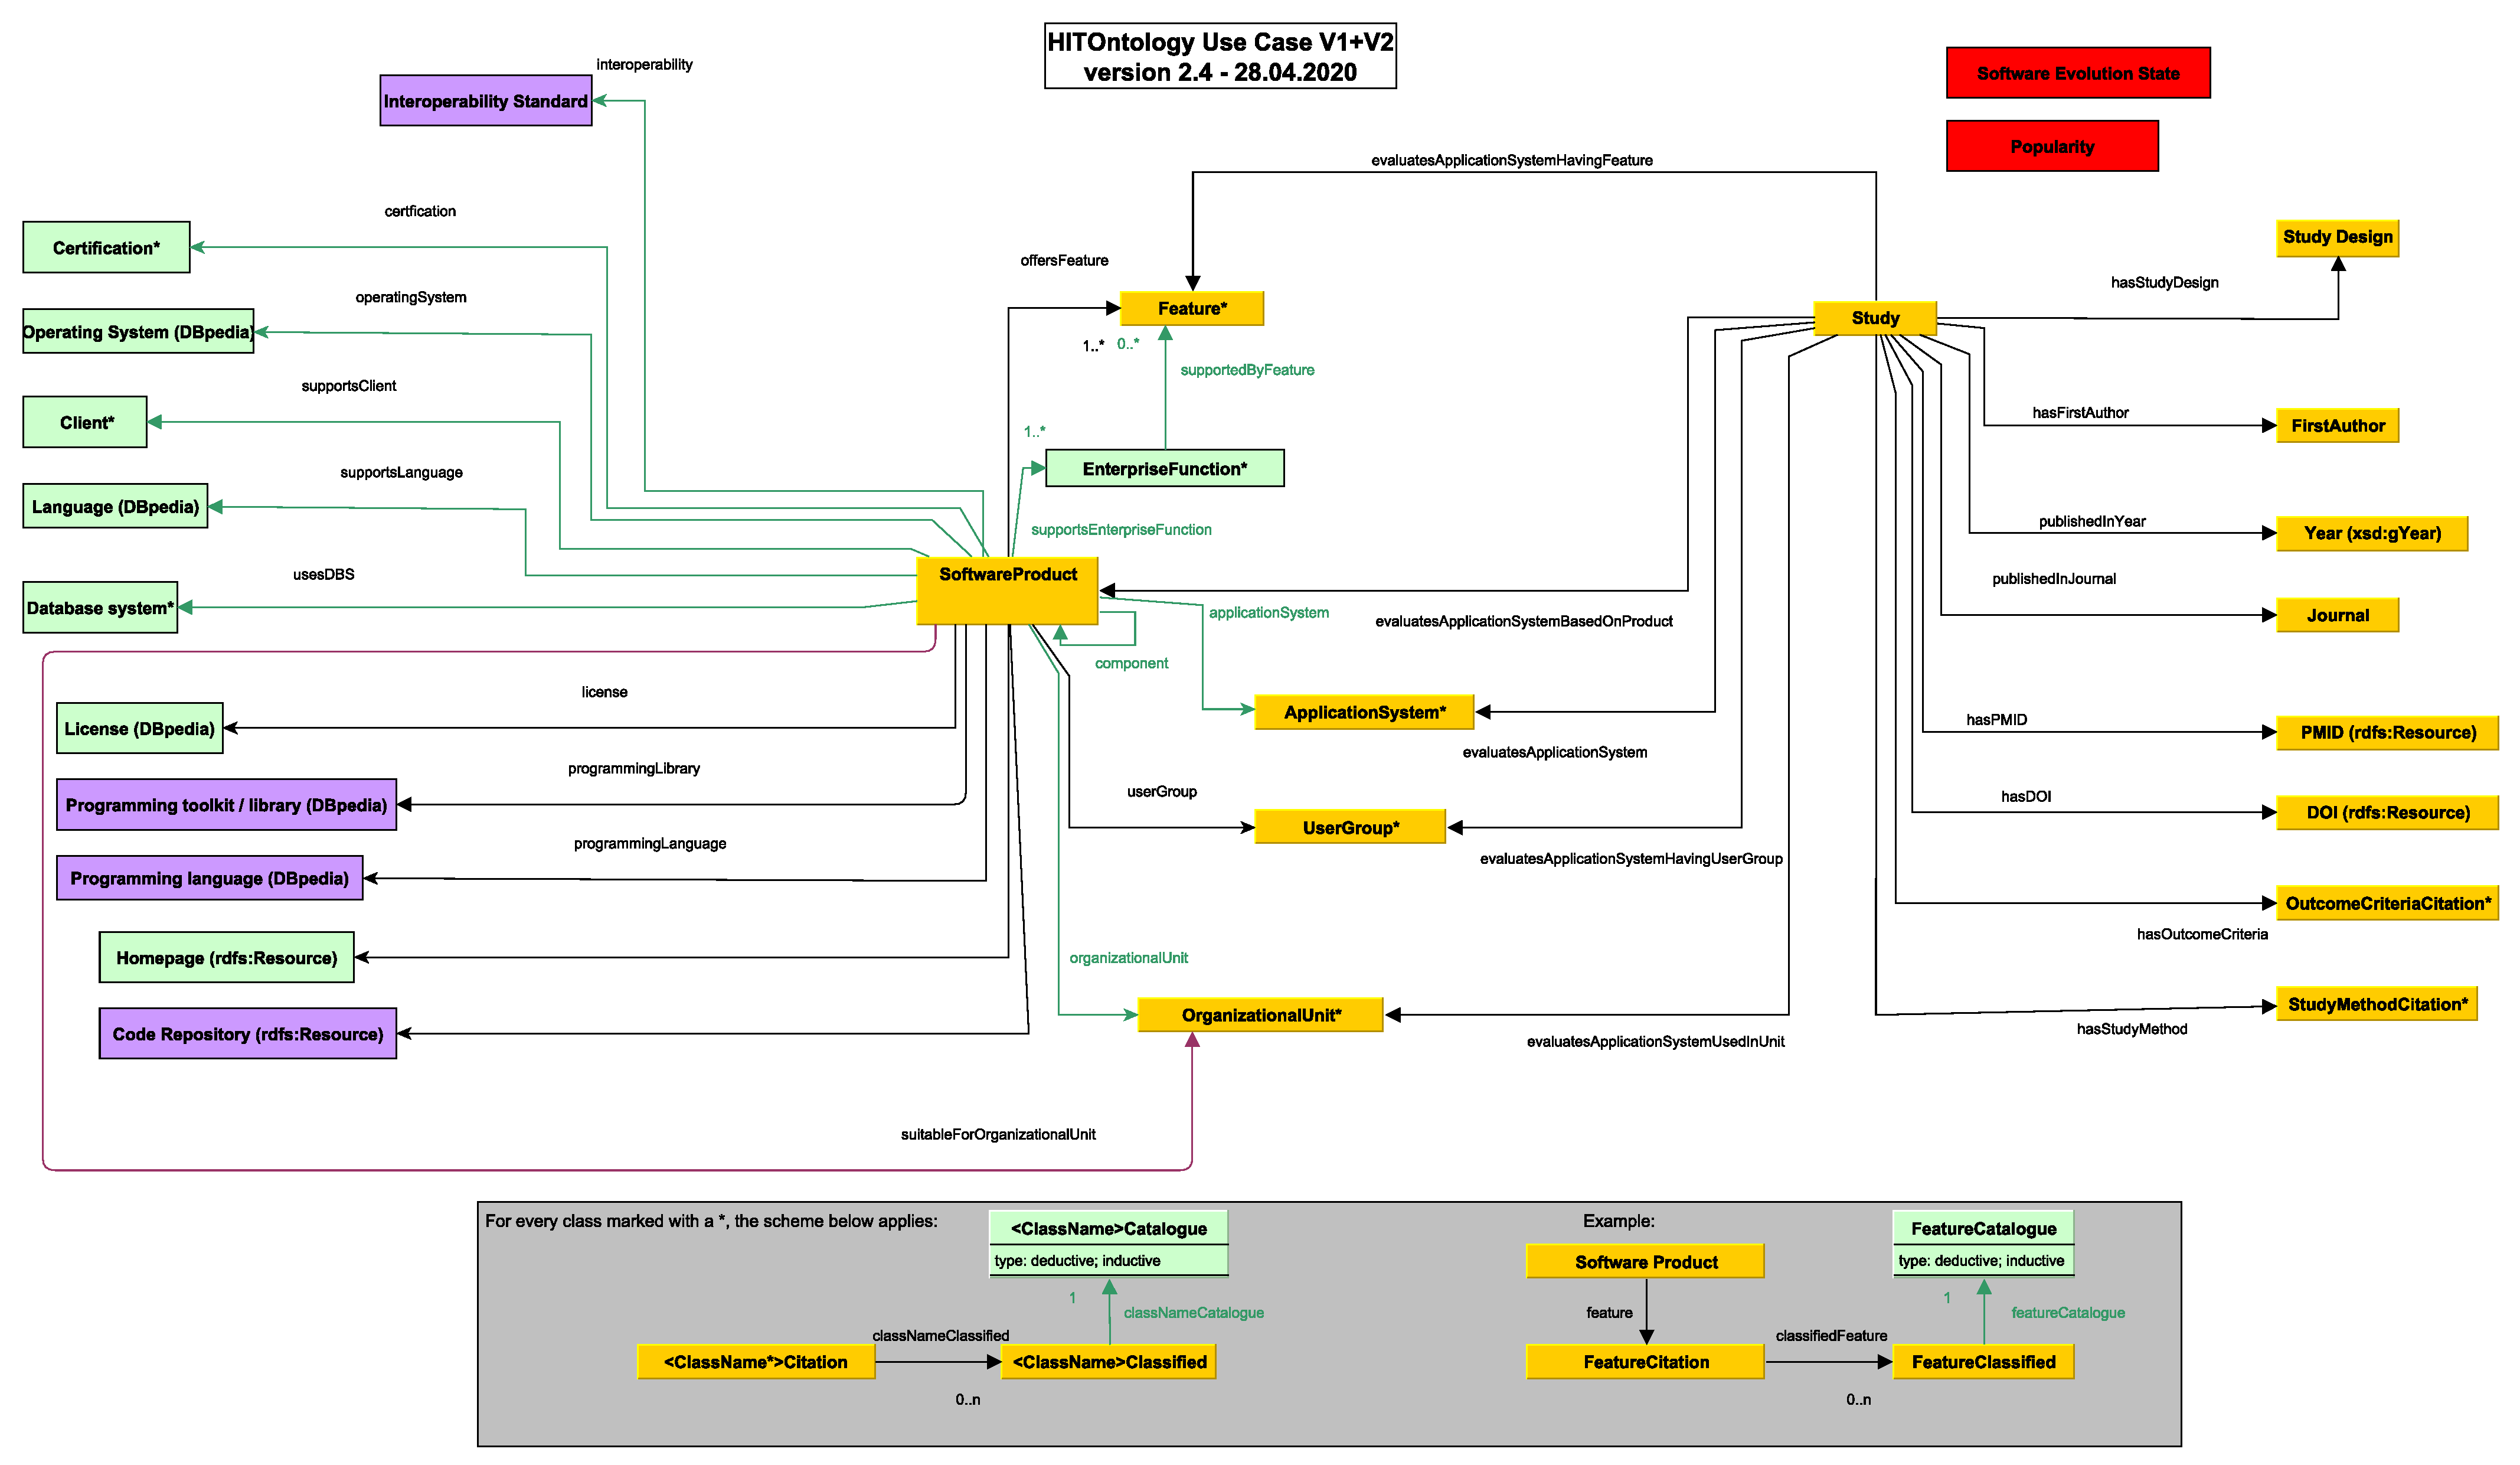
\includegraphics[width=.95\textwidth]{img/HITontology.pdf}
\end{frame}

\begin{frame}{HITO: Merkmale von Softwareprodukten}
\begin{columns}
  \column{0.45\linewidth}
  \begin{itemize}
    \item stimmen größtenteils überein mit Merkmalen, die auf Medfloss.org beschrieben werden
    \item Unterschied: Nutzung von DBpedia-Einträgen als „Kataloge“ für Klassen, z.B.
    \begin{itemize}
      \item Operating System
      \item Language
      \item Programming Language
    \end{itemize}
  \end{itemize}
  \column{0.6\linewidth}
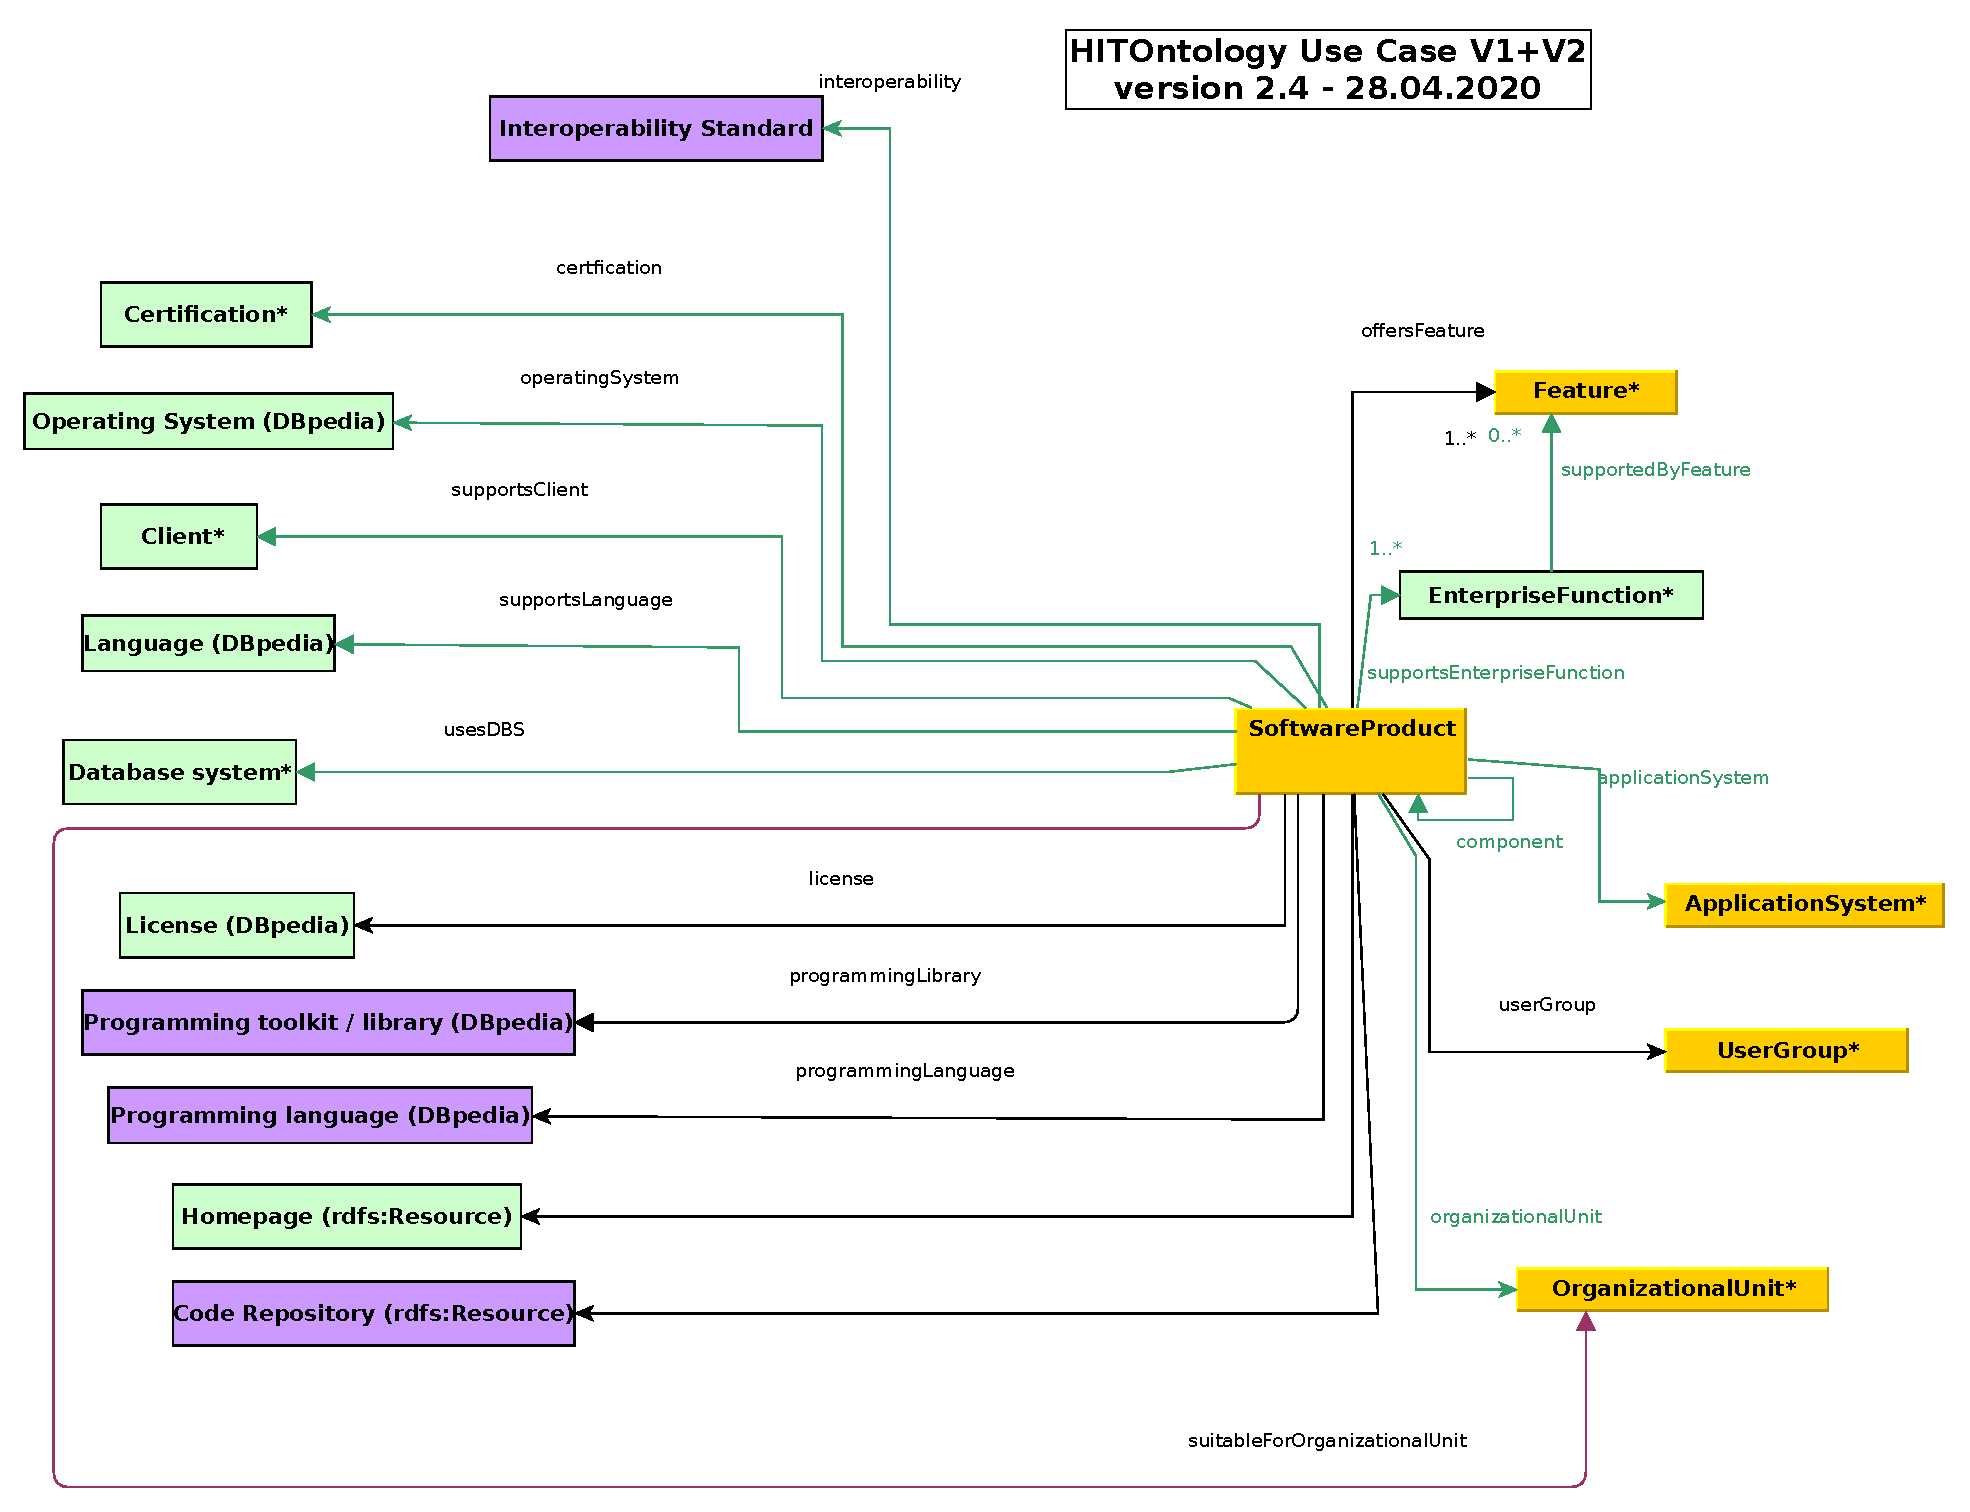
\includegraphics[width=\textwidth]{img/excerpt2.pdf}
\end{columns}
\end{frame}

\begin{frame}{HITO: Unternehmensaufgaben und Features}
\begin{columns}
  \column{0.6\linewidth}
  Softwareprodukte
  \begin{itemize}
    \item unterstützen Unternehmensaufgaben (enterprise functions) im Gesundheitswesen, z.B. \enquote{Patientenverwaltung}, \enquote{Pflegerische Entlassung}
    \item haben Features, z.B. \enquote{Kalenderfunktion}, \enquote{Templates für Berichte}
  \end{itemize}
  \column{0.4\linewidth}
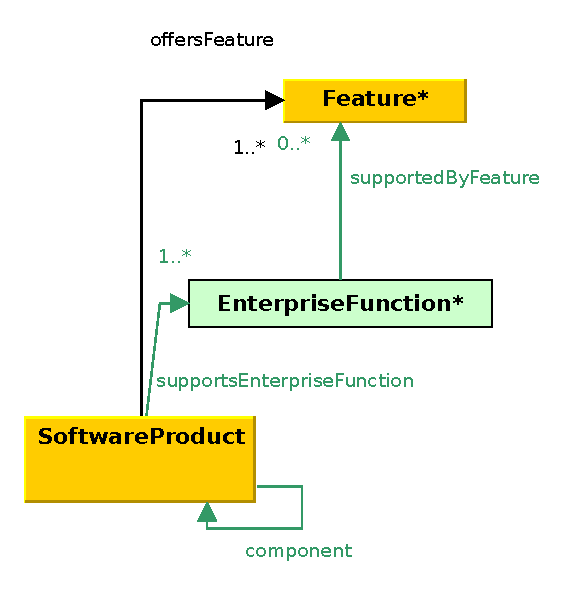
\includegraphics[width=\textwidth]{img/excerpt3.pdf}
\end{columns}
\end{frame}

\begin{frame}{Softwareprodukte und Anwendungssysteme}
\begin{columns}
  \column{0.65\linewidth}
  \begin{itemize}
    \item Softwareprodukte werden durch Adaptation in der Gesundheitseinrichtung zum Anwendungssystem (LIS, RIS, PACS, EPR, ...)
    \item Nutzergruppen sind z.B. Ärzte, Pflegekräfte, Labortechniker
    \item Organisationseinheiten sind z.B. Krankenhaus, Radiologieabteilung, Arztpraxis
  \end{itemize}
  \column{0.4\linewidth}
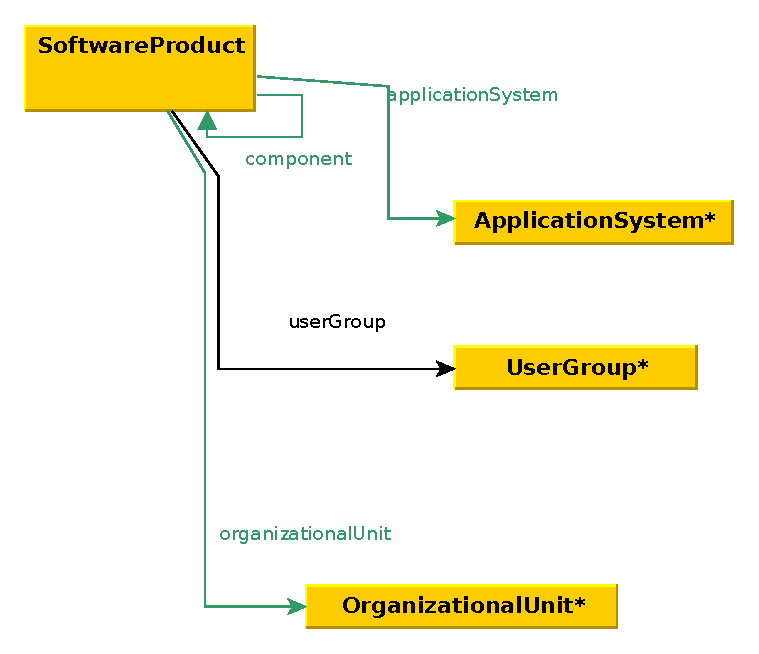
\includegraphics[width=\textwidth]{img/excerpt4.pdf}
\end{columns}
\end{frame}

\begin{frame}{Softwareprodukte \& Evaluationsstudien}
\centering
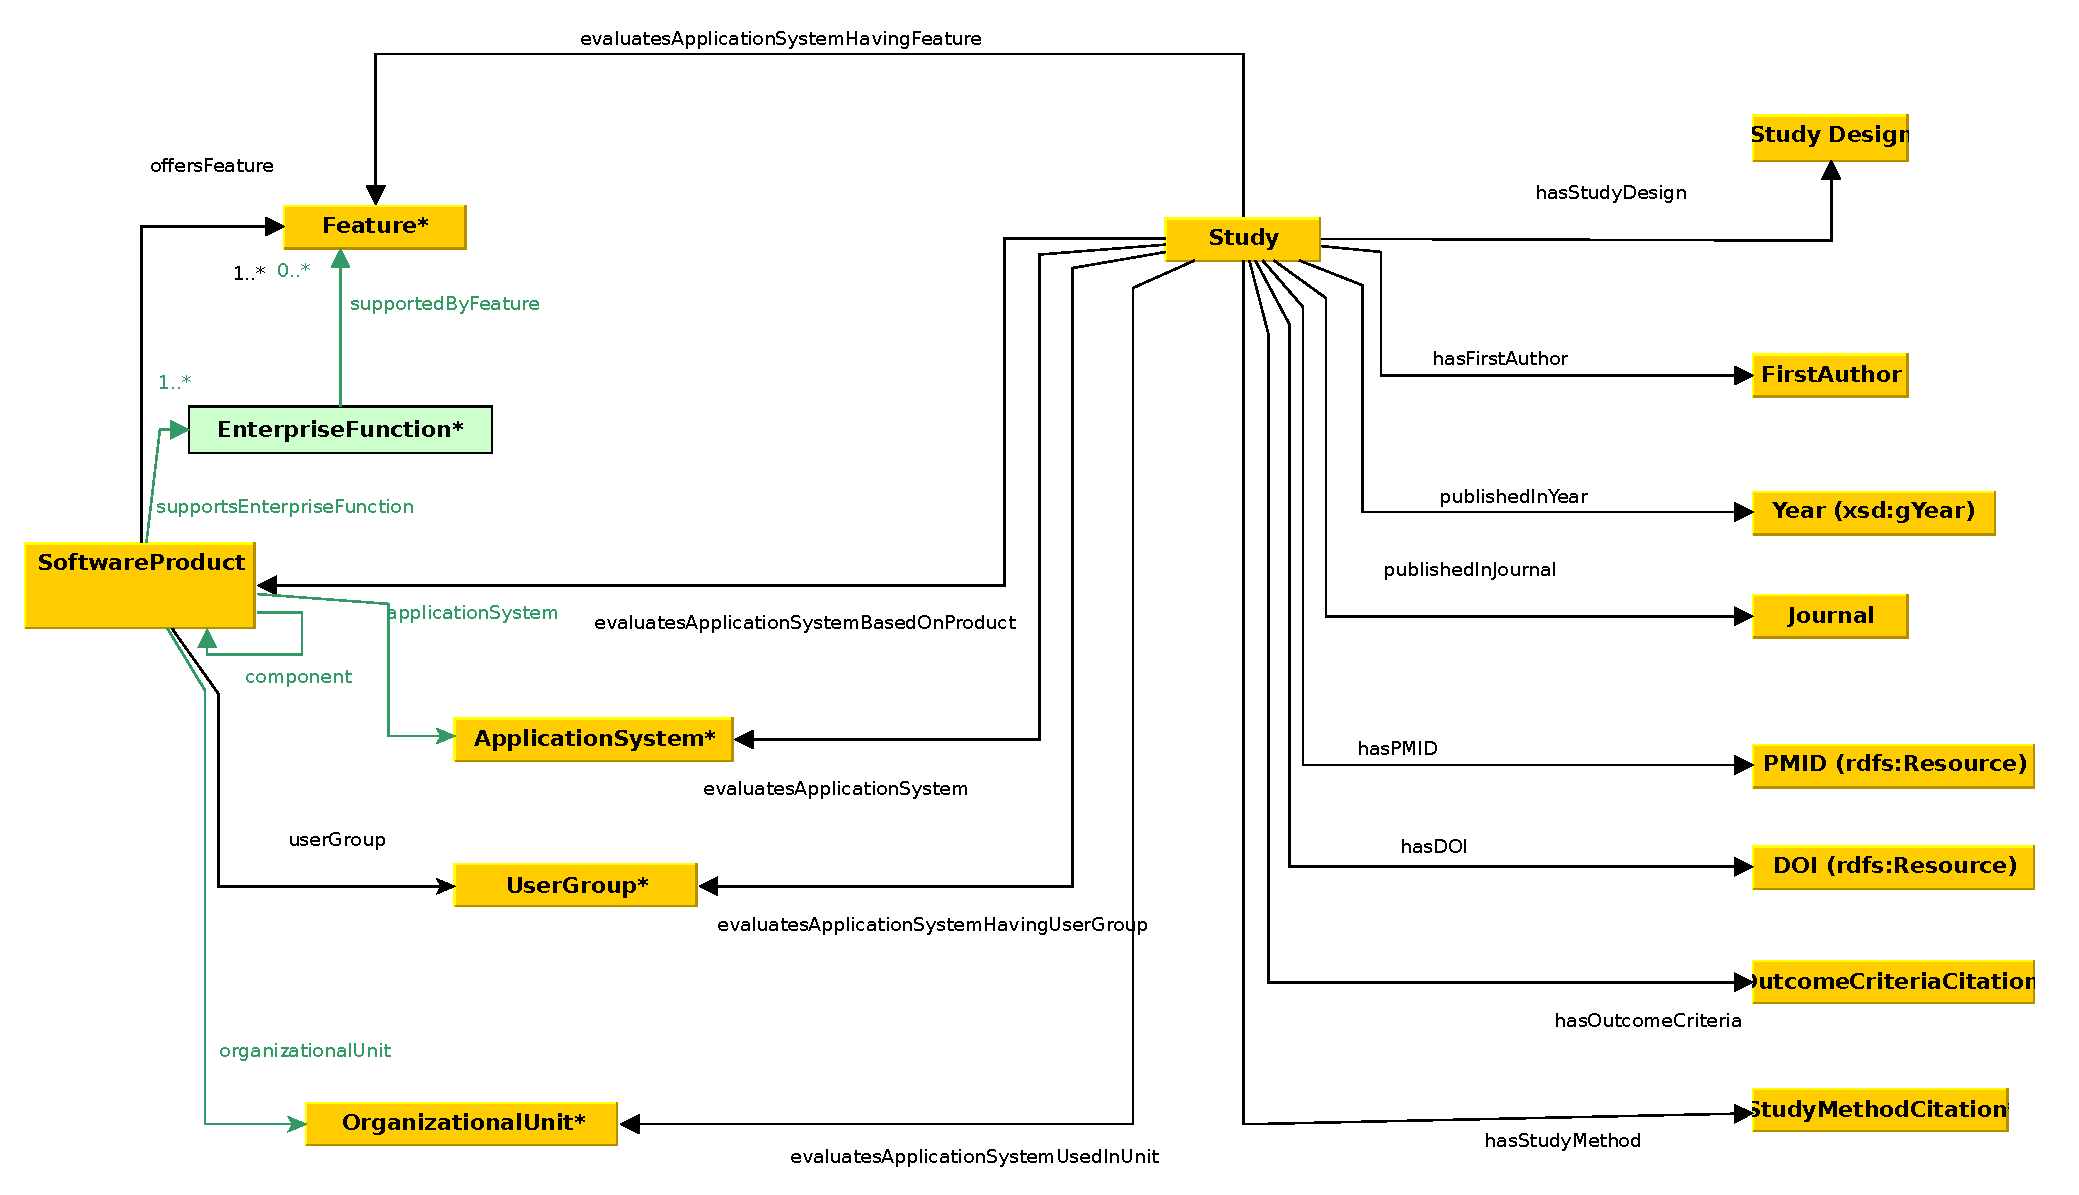
\includegraphics[width=.95\textwidth]{img/excerpt5.pdf}
\end{frame}

\begin{frame}{Fragen?}
  \centering
  \vspace{-0.5cm}
  
\includegraphics[width=\textwidth]{img/fragen.png}
\end{frame}

\begin{frame}{HITO Linked Data Lifecycle}
  \centering
  \vspace{-0.5cm}
  \cycle{mygray}{mygray}{mygray}{mygray}{mygray}{mygray}
\end{frame}

\begin{frame}{HITO Lifecycle Model}
 \centering
  \vspace{-0.5cm}
  \cycle{mypink}{mygray}{mygray}{mygray}{mygray}{mygray}
\end{frame}

\begin{frame}{Eingabemaske für Softwareprodukte: Instance Generator}
\begin{spacing}{1.25}
\begin{itemize}
\item praktische Eingabemaske für MEDFLOSS Softwareprodukte
\item keine Linked Data Vorkenntnisse nötig
\item verfügbar als GitHub Page unter:
\begin{itemize}
\item \url{https://hitontology.github.io/instancegenerator/}
\end{itemize}
\item Modellierung detaillierter Charakteristika
\item Softwareprodukte werden mit allen Eigenschaften in die Ontologie übertragen
\item Nutzung von externen Wissensbasen und individuellen Katalogen
\item Video-Demonstration auf dem HITO YouTube-Kanal:
\begin{itemize}
\item \url{https://youtu.be/EWvEaSCo3Vg}
\end{itemize}
\end{itemize}
\end{spacing}
\end{frame}

\begin{frame}{Fragen?}
  \centering
  \vspace{-0.5cm}
  
\includegraphics[width=\textwidth]{img/fragen.png}
\end{frame}

\begin{frame}{Catalogues and citations -- Example: Bahmni}
  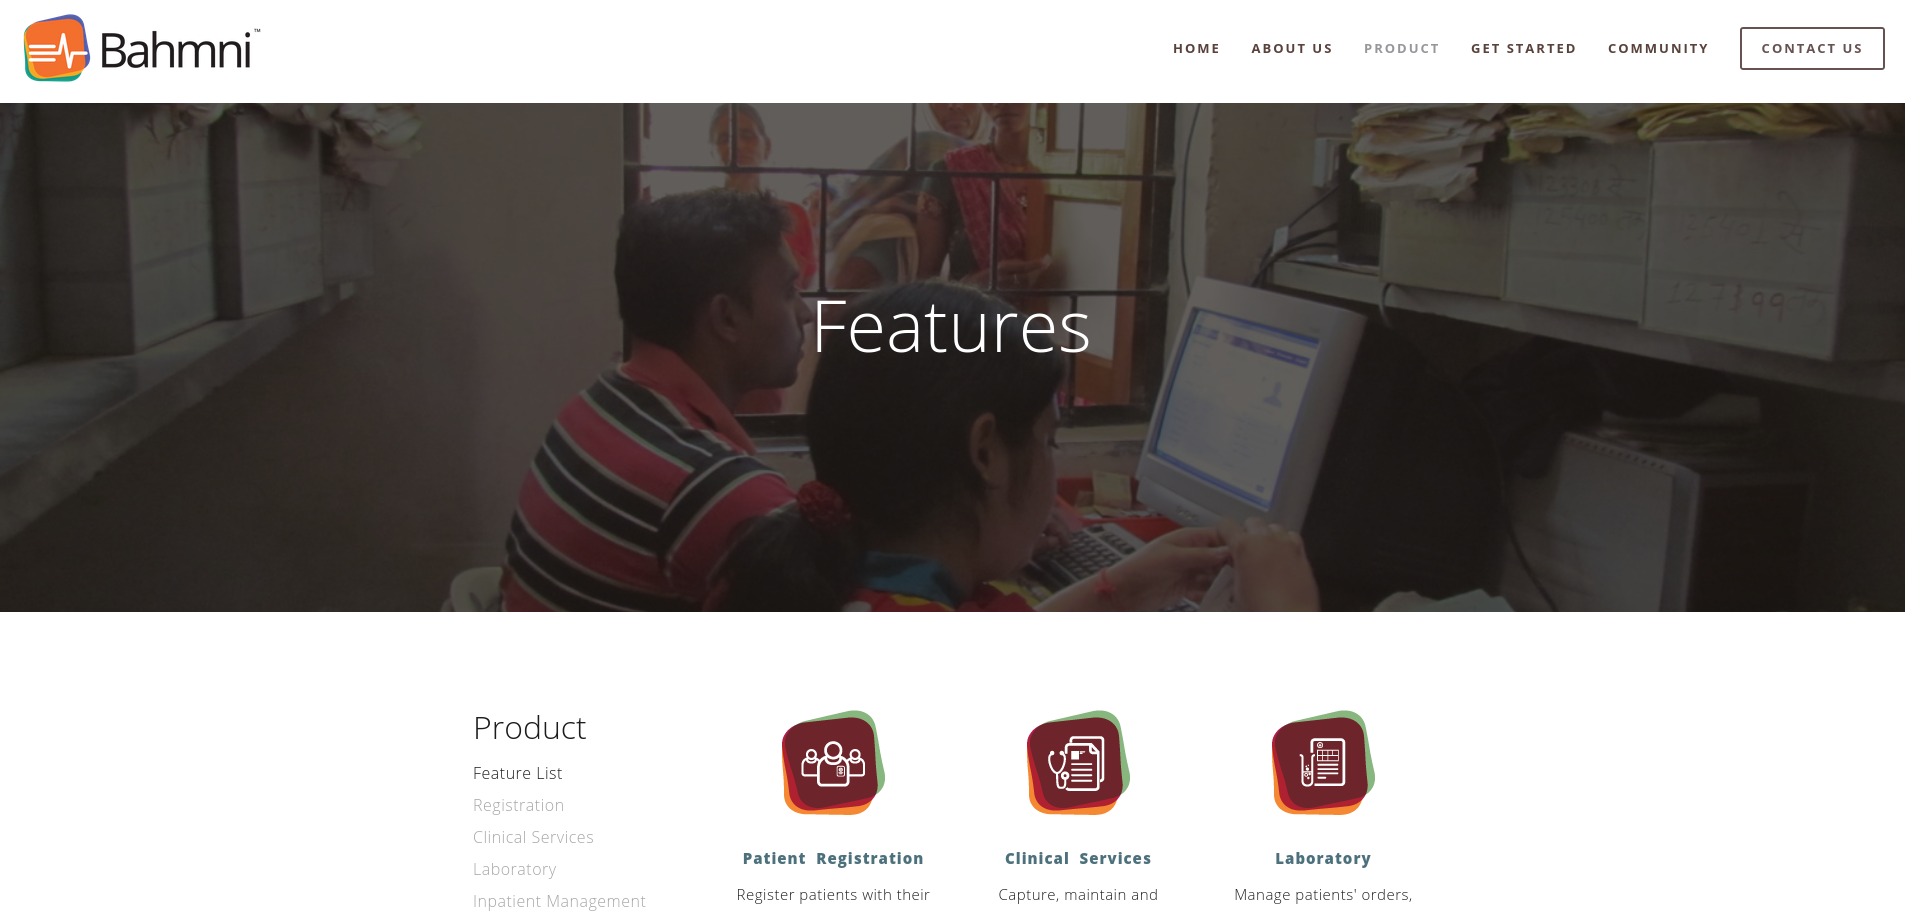
\includegraphics[width=\textwidth]{img/bahmni-example1.png}
\end{frame}

\begin{frame}{Catalogues and citations -- Example: Bahmni}
  \centering
  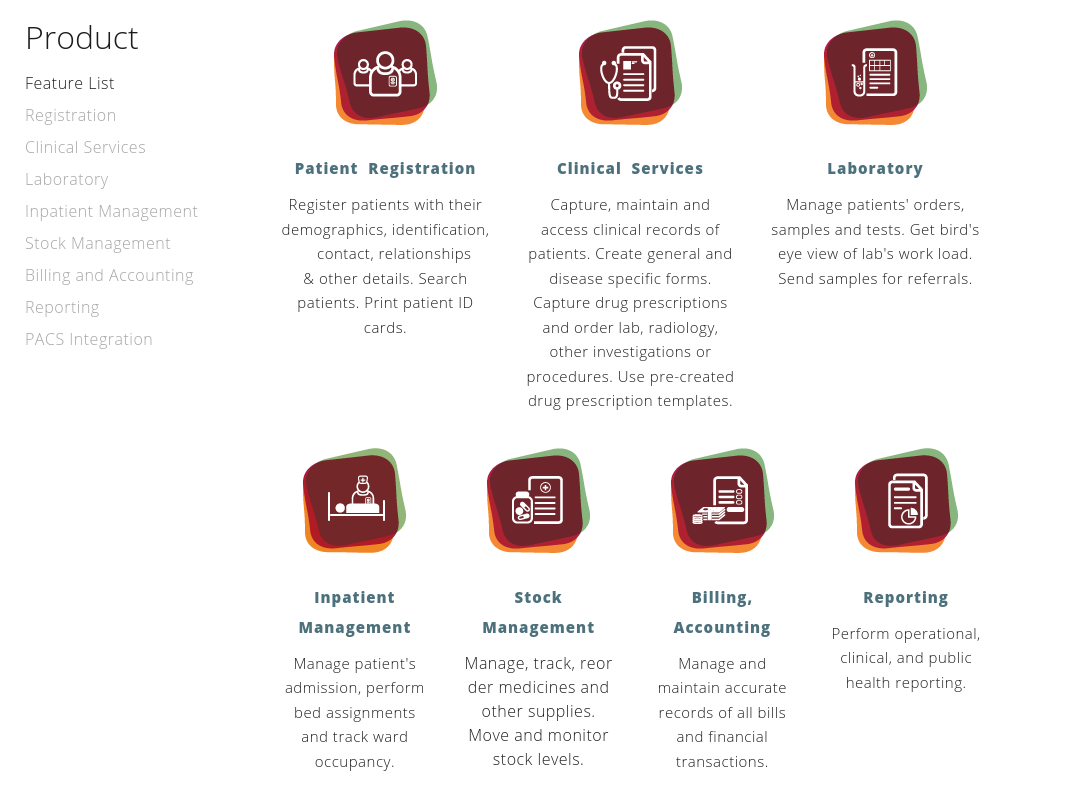
\includegraphics[height=.8\textheight]{img/bahmni-example2.png}
\end{frame}

\begin{frame}{Catalogues and citations -- Example: Bahmni}
  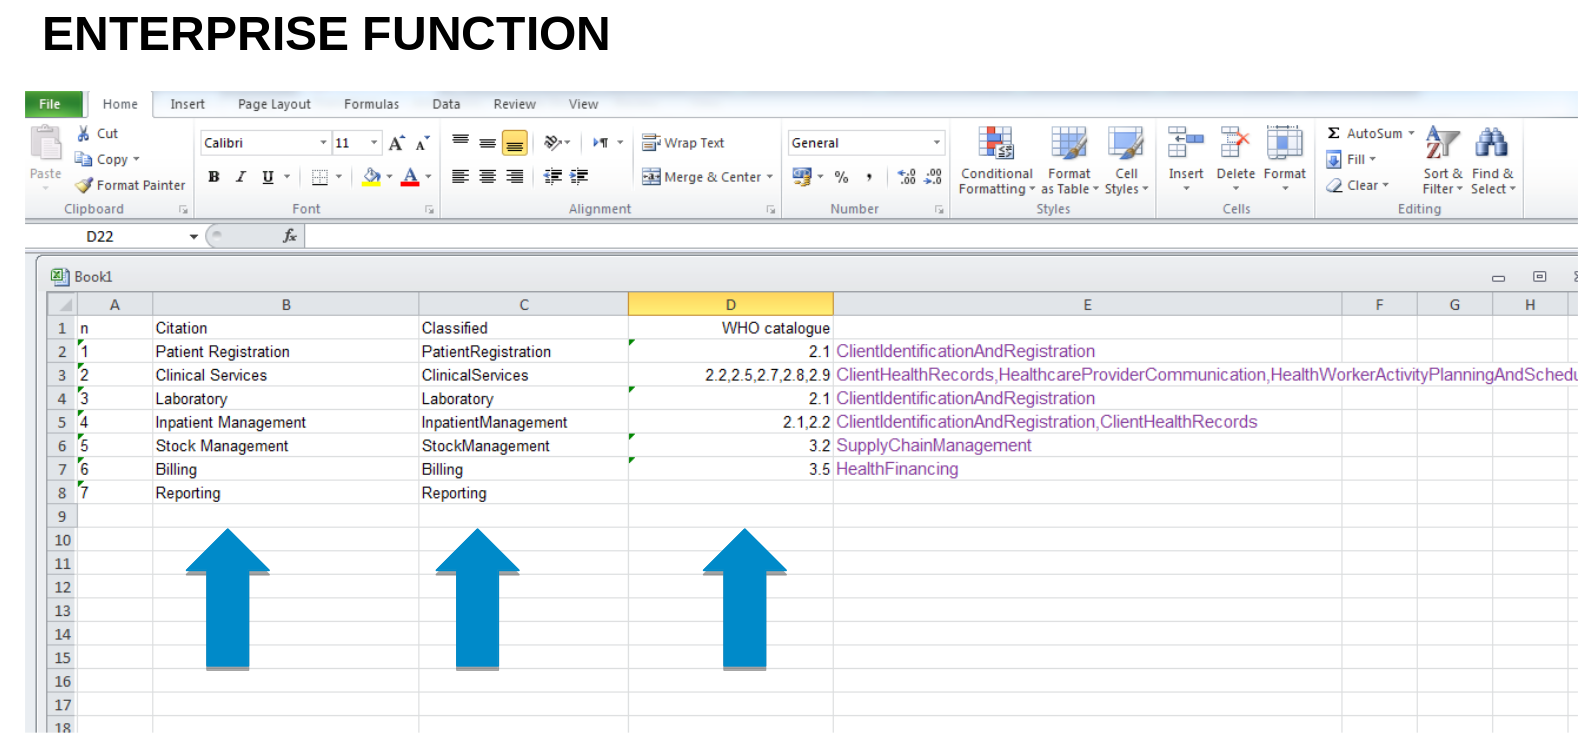
\includegraphics[width=\textwidth]{img/bahmni-table1.png}
\end{frame}

\begin{frame}{Catalogues and citations -- Example: Bahmni}
  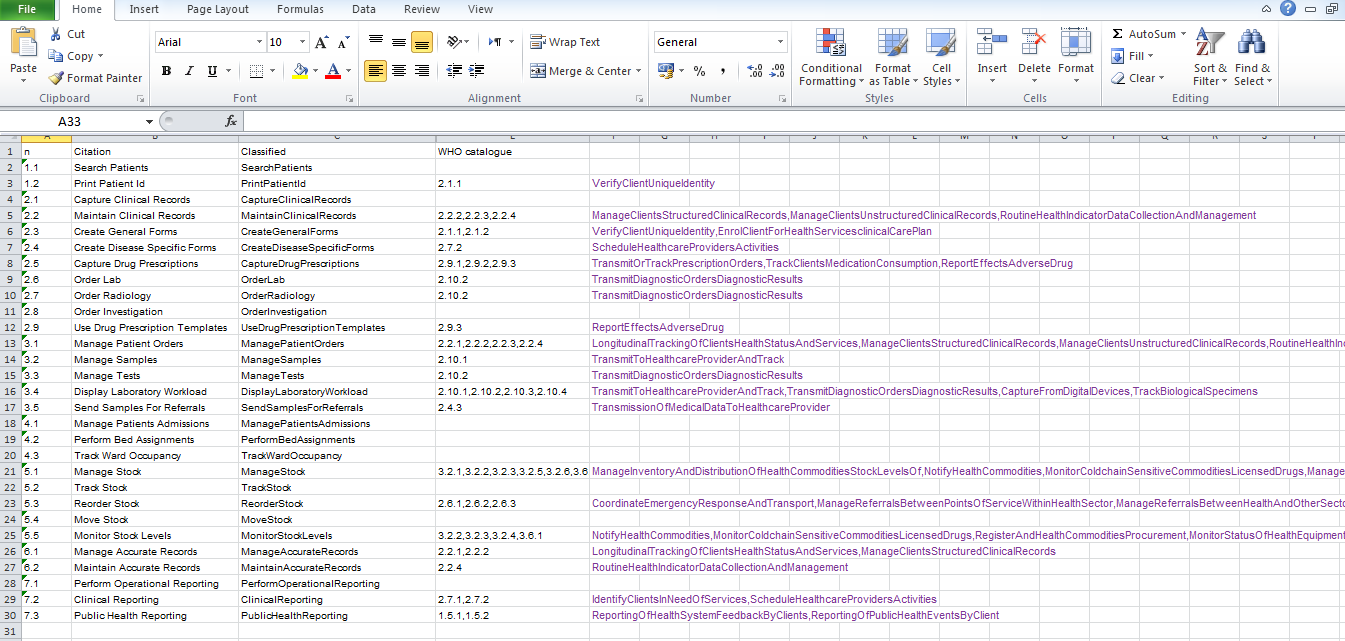
\includegraphics[width=\textwidth]{img/bahmni-table2.png}
\end{frame}

\begin{frame}{Catalogues and citations}
\centering
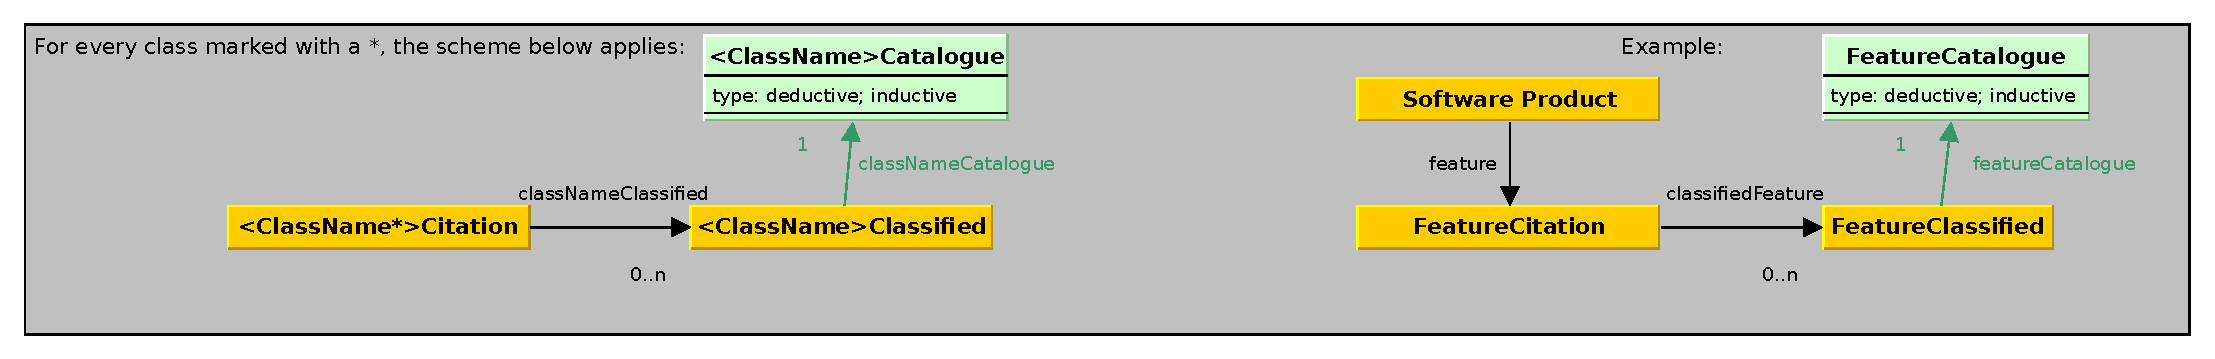
\includegraphics[width=\textwidth]{img/excerpt1.pdf}
\end{frame}

\begin{frame}{Catalogues and citations}
\begin{columns}
  \column{.4\linewidth}
  \vspace{-1cm}
  \begin{spacing}{1.25}
    \begin{itemize}
      \item \emph{Our five catalogue types}
      \begin{itemize}
        \item Application System
        \item Enterprise Function
        \item Feature
        \item User Group
        \item Organizational Unit
      \end{itemize}
    \end{itemize}
  \end{spacing}
  \column{.5\linewidth}
  \centering
  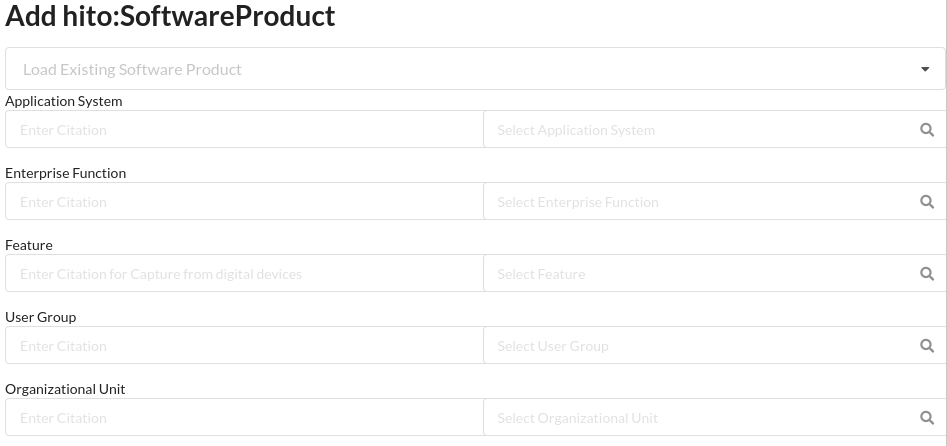
\includegraphics[width=\textwidth]{img/iglook.png}
\end{columns}
\end{frame}

\begin{frame}{Catalogue Sources}
  \begin{columns}
    \column{0.3\linewidth}
    
\includegraphics[width=\textwidth]{img/WHOLogo.pdf}
    \column{0.6\linewidth}
    
\includegraphics[width=\textwidth]{img/dhi.png}
\end{columns}
\end{frame}

\begin{frame}{WHO -- DHI}
\begin{columns}
  \column{0.5\linewidth}
  \vspace{0.5cm}
  \centering
  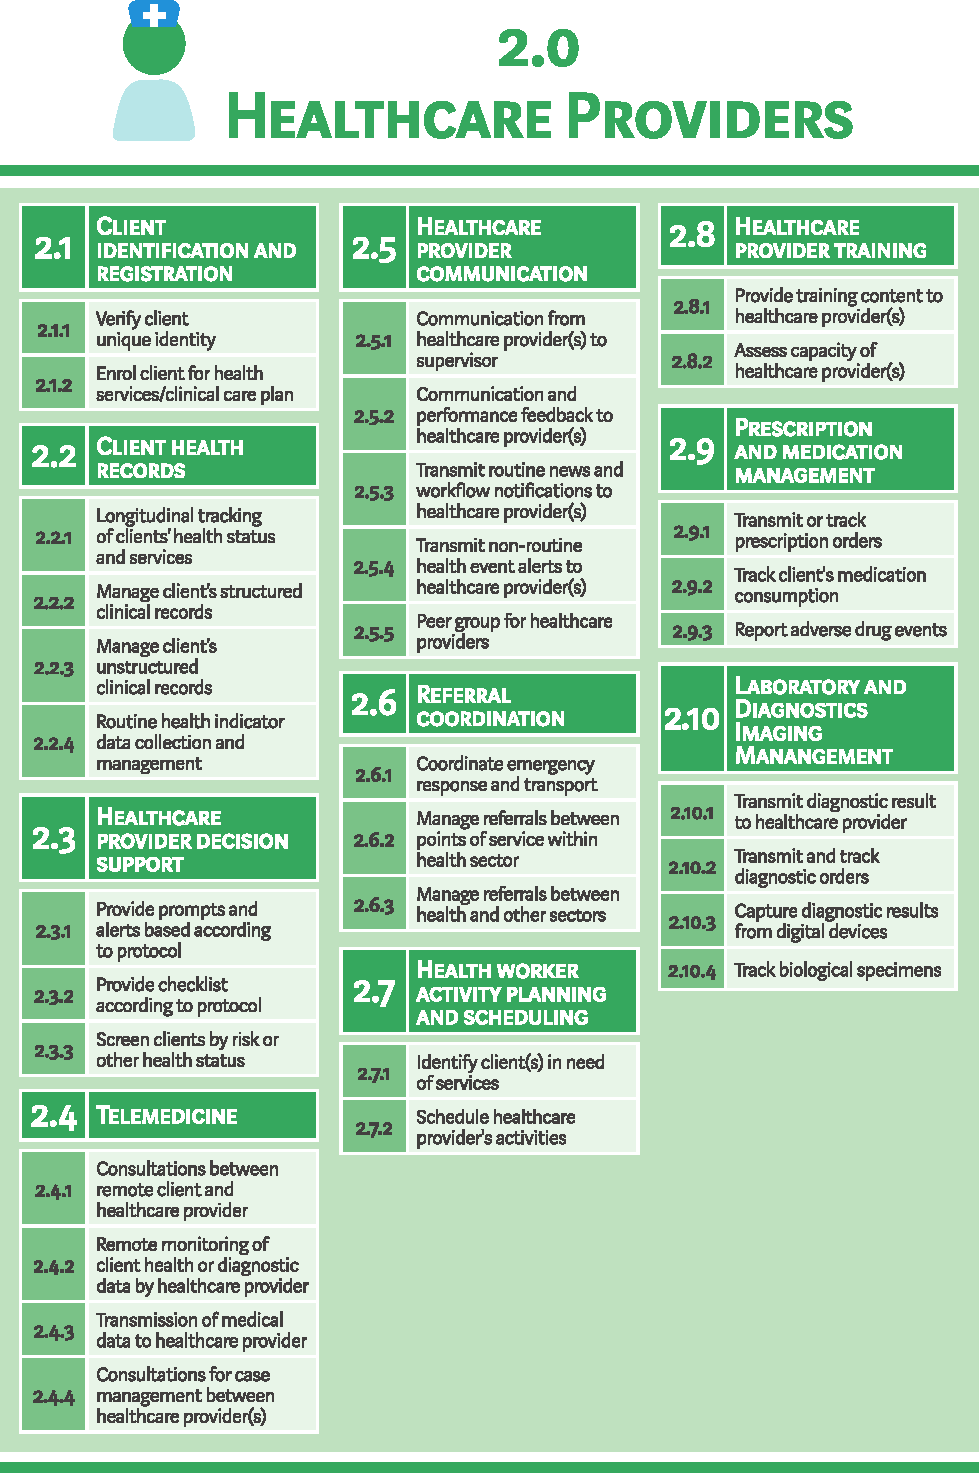
\includegraphics[height=.8\textheight]{img/whodhi-providers.pdf}
  \column{0.5\linewidth}
  \vspace{0.5cm}
  \centering
  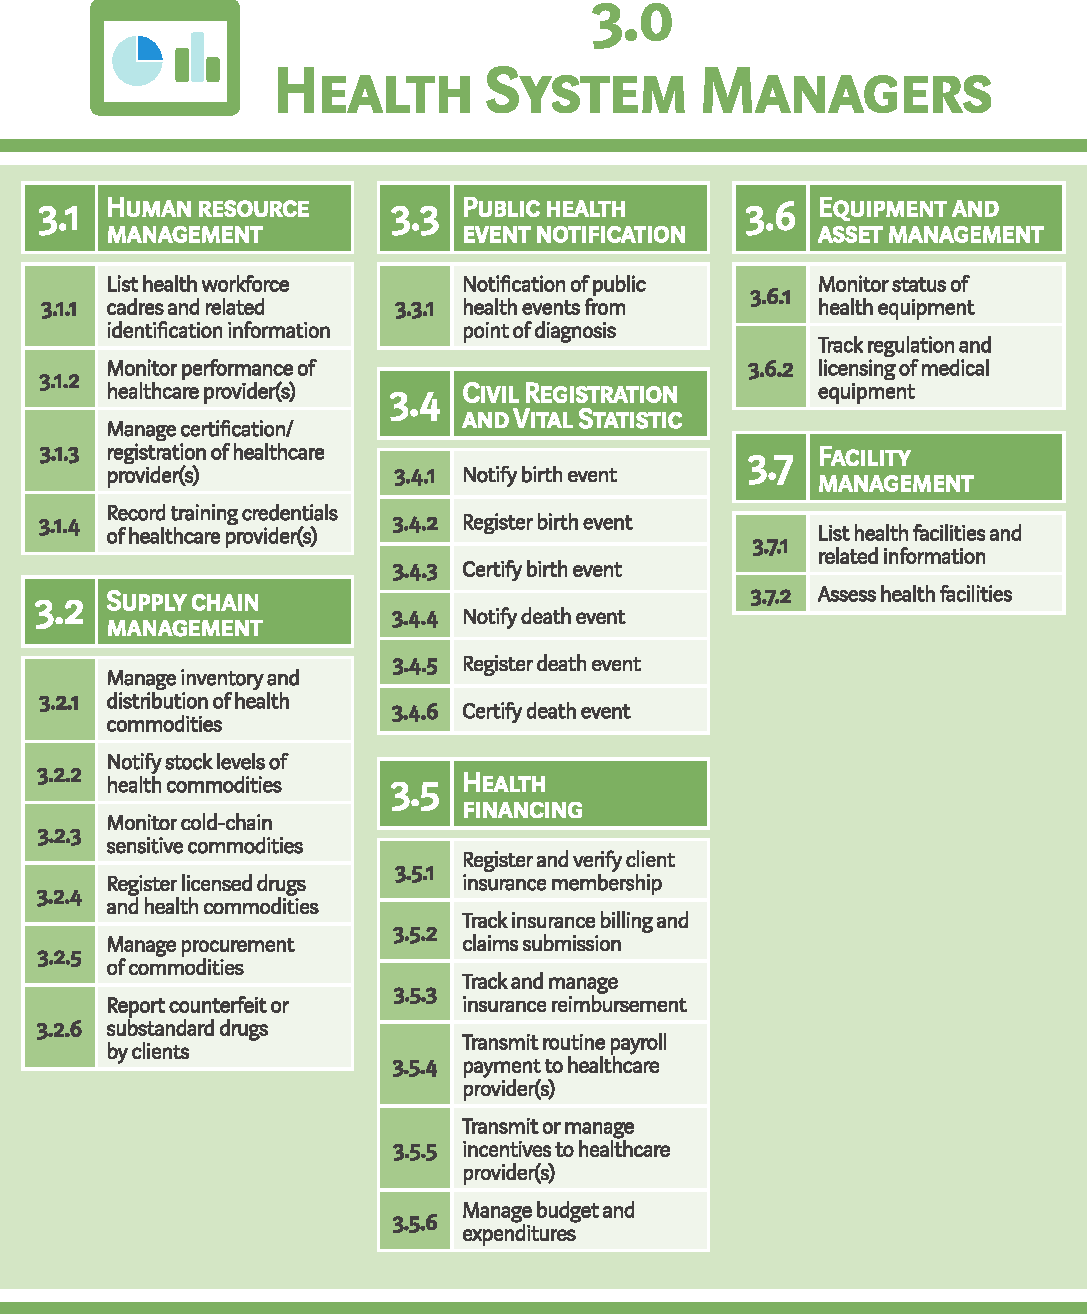
\includegraphics[height=.8\textheight]{img/whodhi-managers.pdf}
\end{columns}
\end{frame}

\begin{frame}{Catalogue Sources -- The \enquote{Blue Book}}
\begin{columns}
  \column{0.5\linewidth}
  \vspace{0.5cm}
  \centering
  
\includegraphics[height=.8\textheight]{img/bb-cover.jpg}
  \column{0.5\linewidth}
  \vspace{0.5cm}
  \centering
  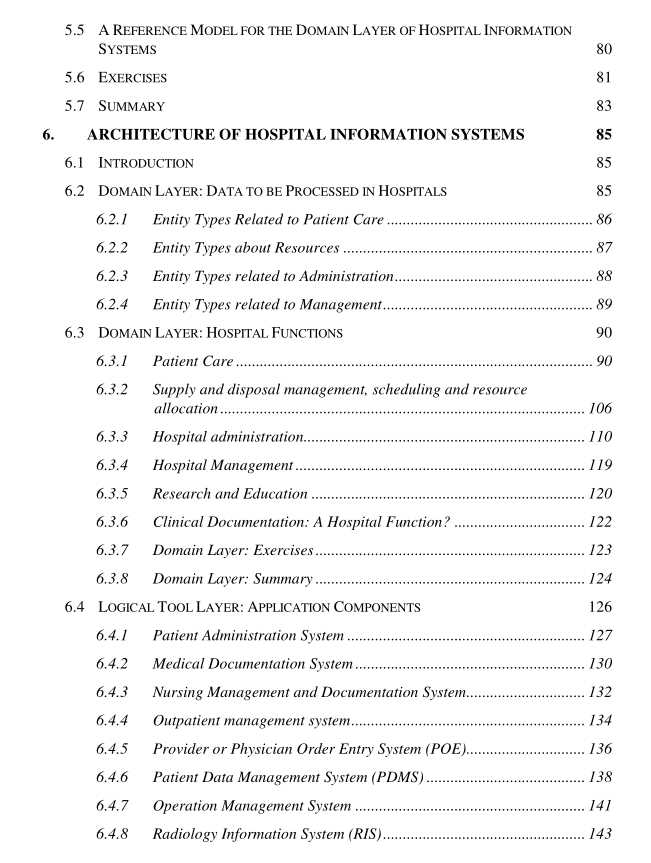
\includegraphics[width=.9\textwidth,height=.8\textheight]{img/bb-content.png}
\end{columns}
\end{frame}

\begin{frame}{Catalogue Sources}
  \centering
  \large Health Information Systems (A.Winter et al.) (\enquote{Blue Book})
  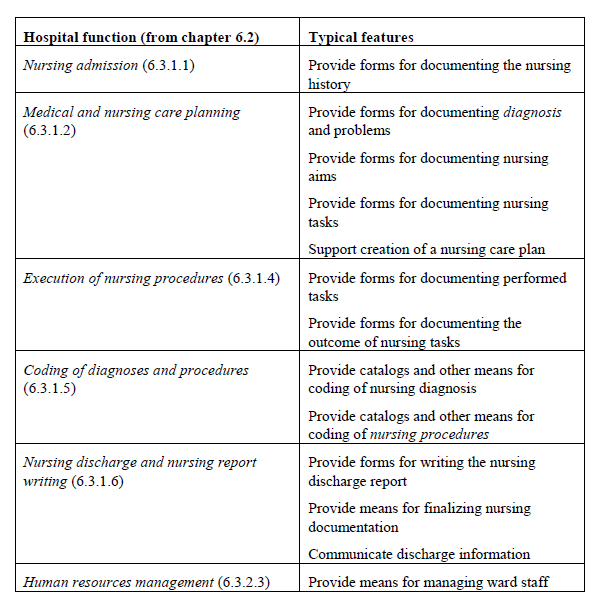
\includegraphics[height=.7\textheight]{img/bb-table.png}
\end{frame}

\begin{frame}{Reference model for the domain layer of hospital information systems (Enterprise functions)}
  \centering
  \vspace{-0.3cm}
  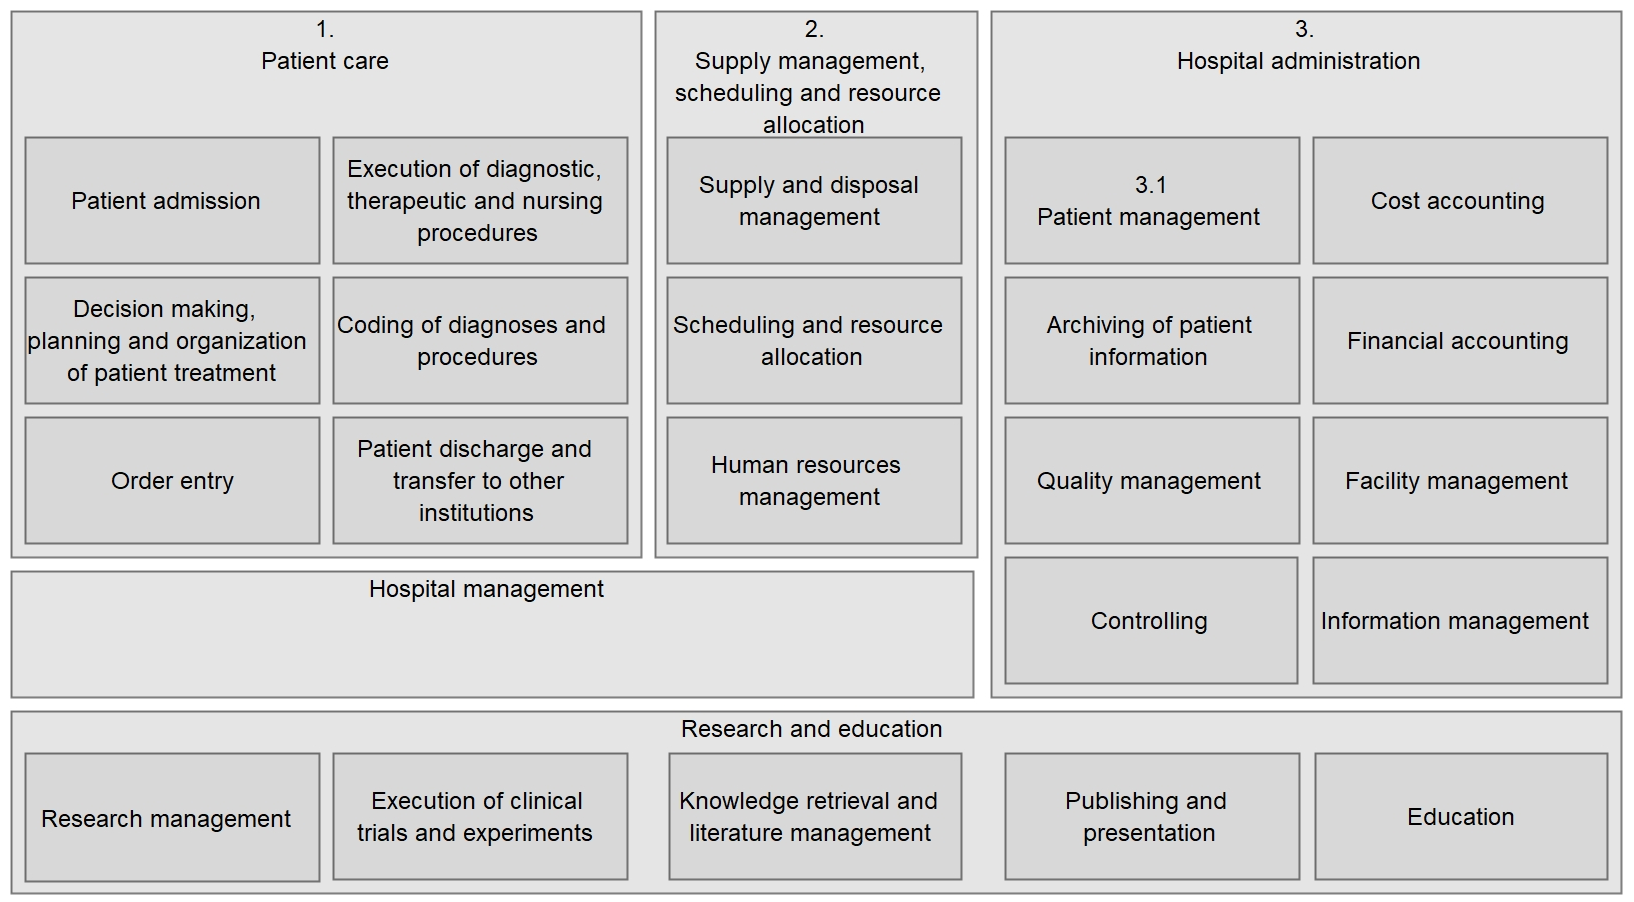
\includegraphics[width=.95\textwidth]{img/rmdl.png}
\end{frame}

\begin{frame}{Catalogue Sources}
\begin{spacing}{1.5}
  Other Catalogue Sources
  \begin{itemize}
    \item SNOMED CT for User Groups and Organizational Units
    \item \emph{HL7 EHR-S Functional Model}
  \end{itemize}
\end{spacing}
\end{frame}

\begin{frame}{Application System Catalogues}
\begin{spacing}{1.5}
  \emph{Application System Catalogues:}
  \begin{itemize}
    \item WHO-DHI System Category
    \item BB Application Component
    \item BB Architecture
  \end{itemize}
\end{spacing}
\end{frame}

\begin{frame}{Enterprise Function Catalogues}
\begin{spacing}{1.5}
  \emph{Enterprise Function Catalogues:}
  \begin{itemize}
    \item BB Architecture
    \item BB Reference Model
  \end{itemize}
  \end{spacing}
\end{frame}

\begin{frame}{Feature Catalogues}
\begin{spacing}{1.5}
  \emph{Feature Catalogues:}
  \begin{itemize}
    \item WHO-DHI Health System Managers
    \item WHO-DHI Healthcare Provider Feature Catalogue
    \item WHO-DHI Client Feature Catalogue
    \item WHO-DHI Data Service
    \item BB Architecture
  \end{itemize}
  \end{spacing}
\end{frame}

\begin{frame}{User Group \& Organizational Unit Catalogues}
\begin{spacing}{1.5}
  \emph{User Group \& Organizational Unit Catalogues:}
  \begin{itemize}
    \item SNOMED CT
  \end{itemize}
  \end{spacing}
\end{frame}

\begin{frame}{Fragen?}
  \centering
  \vspace{-0.5cm}
  
\includegraphics[width=\textwidth]{img/fragen.png}
\end{frame}

\begin{frame}{HITO Lifecycle Storage \& Query}
 \centering
  \vspace{-0.5cm}
  \cycle{mygreen}{mypink}{mypink}{mygray}{mygray}{mygray}
\end{frame}

\begin{frame}{Wie geht es weiter?}
  \begin{spacing}{1.5}
    Was passiert mit den Daten, die mittels des Instance Generators modelliert wurden?
  \begin{itemize}
    \item Speicherung und Versionskontrolle durch GitHub Repository
    \item Datenbestand in SPARQL-Endpoint, Äquivalent zur Datenbank
  \end{itemize}
\end{spacing}
\end{frame}

\begin{frame}{HITO Lifecycle Browse}
  \centering
  \vspace{-0.5cm}
  \cycle{mygreen}{mygreen}{mygreen}{mypink}{mygray}{mygray}
\end{frame}

\begin{frame}{Software Products in HITO Ontology (with LODView)}
\centering
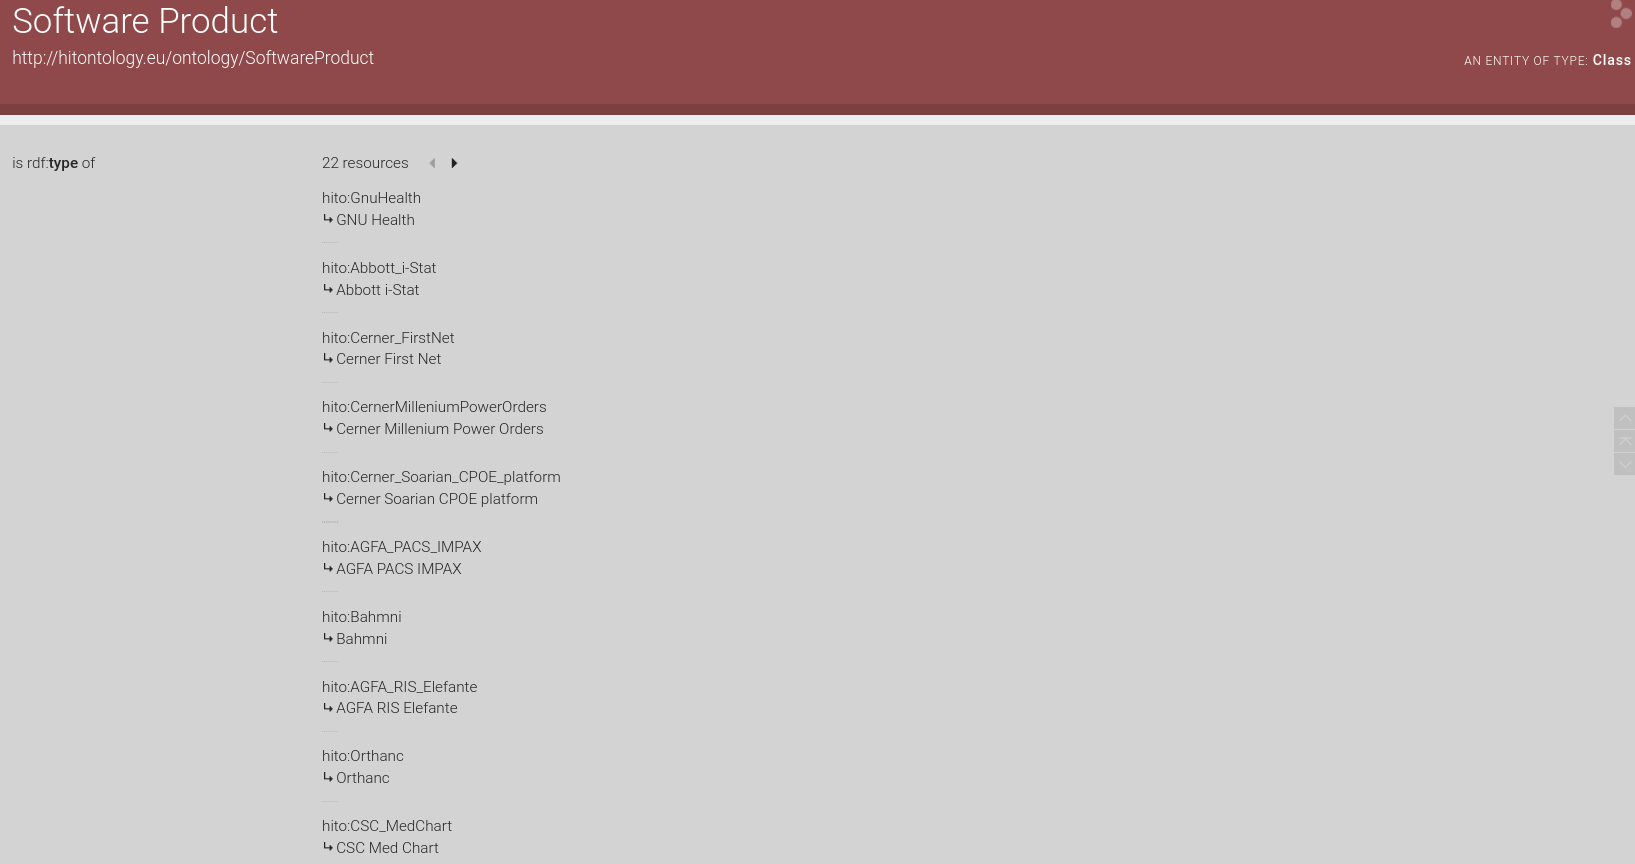
\includegraphics[width=\textwidth]{img/softwareproduct.png}
\end{frame}

\begin{frame}{Beispiel I: GNU Health in LODView}
\vspace{-0.3cm}
\centering
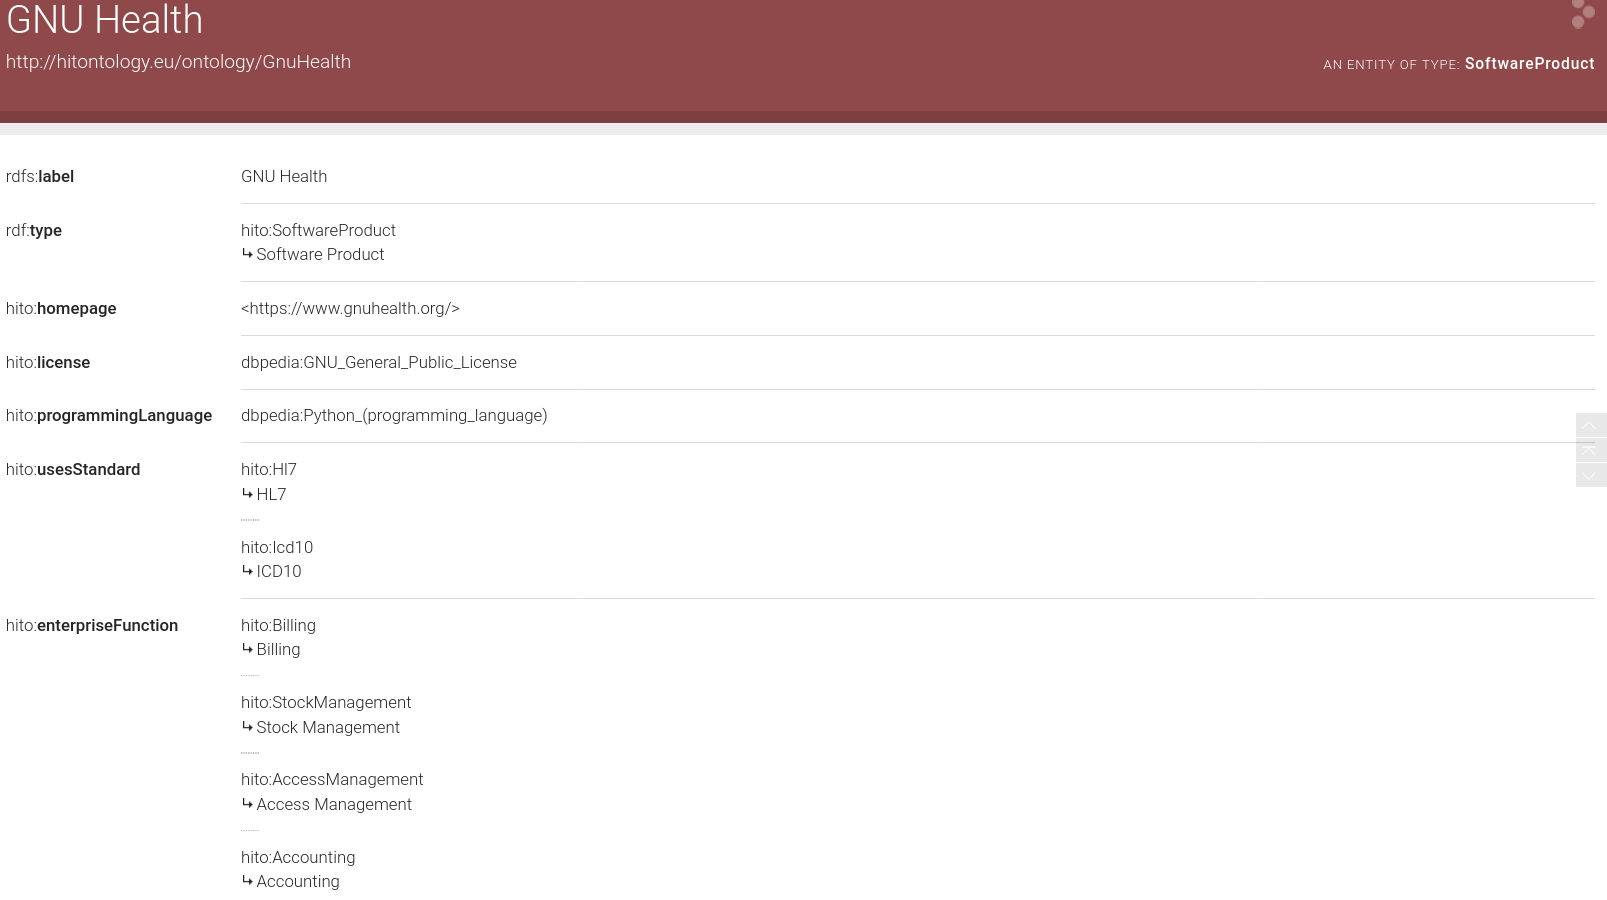
\includegraphics[width=.95\textwidth]{img/GnuHealth.png}
\footnotesize{\url{https://hitontology.eu/ontology/GnuHealth}}
\end{frame}

\begin{frame}{Beispiel II: Bahmni in LODView}
\vspace{-0.3cm}
\centering
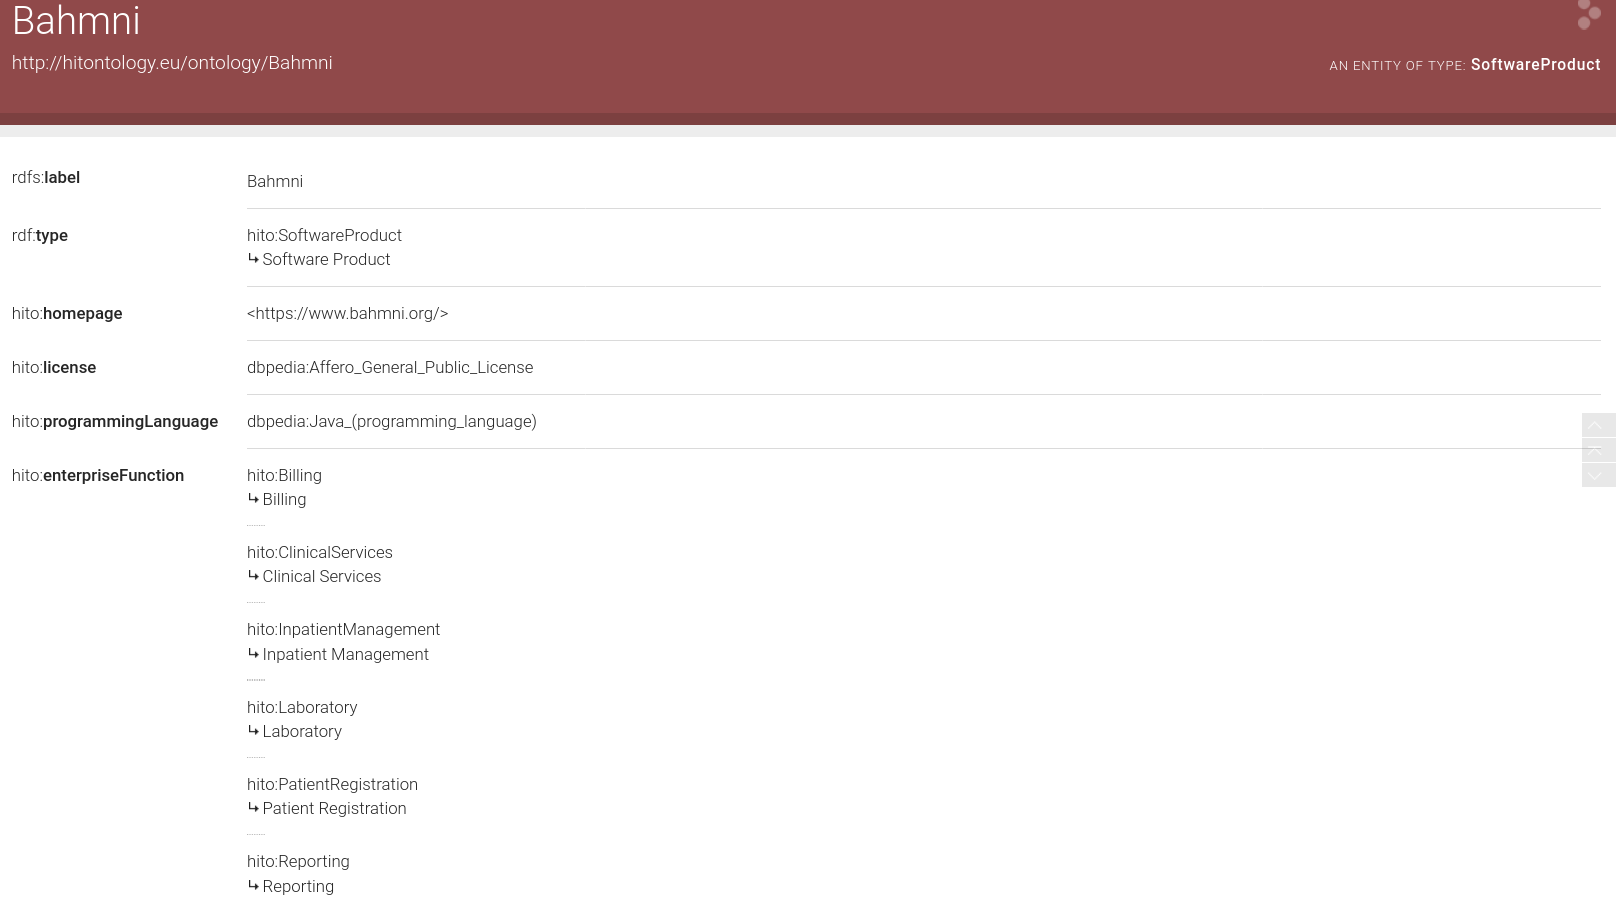
\includegraphics[width=.95\textwidth]{img/bahmni.png}
\footnotesize{\url{https://hitontology.eu/ontology/Bahmni}}
\end{frame}

\begin{frame}{HITO Lifecycle Search/Explore}
  \centering
  \vspace{-0.5cm}
  \cycle{mygreen}{mygreen}{mygreen}{mygreen}{mypink}{mygray}
\end{frame}

\begin{frame}{Kriteriensuche nach Studien -- Faceted Search}
\centering
\vspace{-0.3cm}
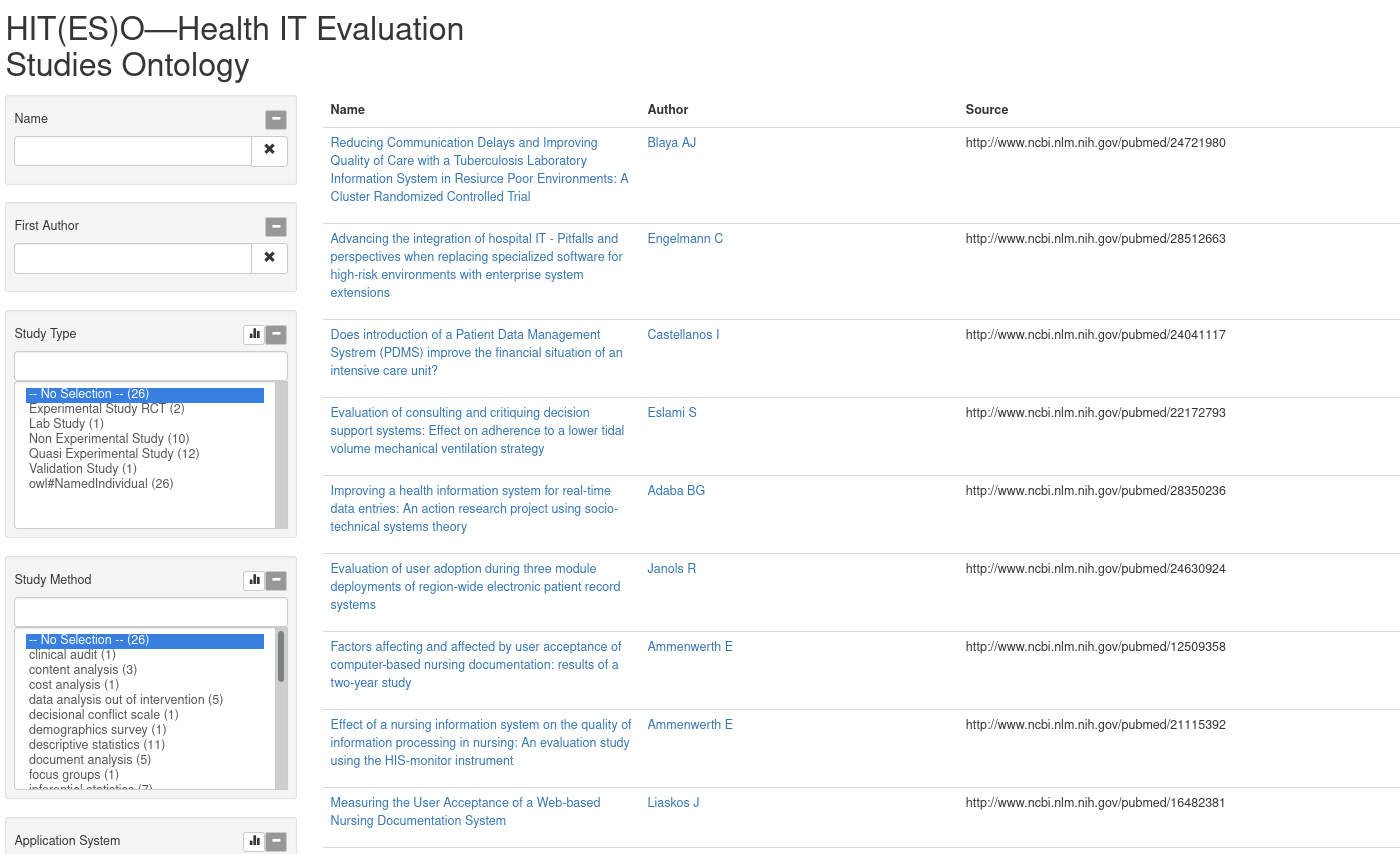
\includegraphics[height=.8\textheight]{img/facetedsearch.png}
\vspace{0.3cm}
\footnotesize{\url{https://hitontology.eu/search/}}
\end{frame}

\begin{frame}{Beispiel II: Bahmni als Graph (Ausschnitt)}
  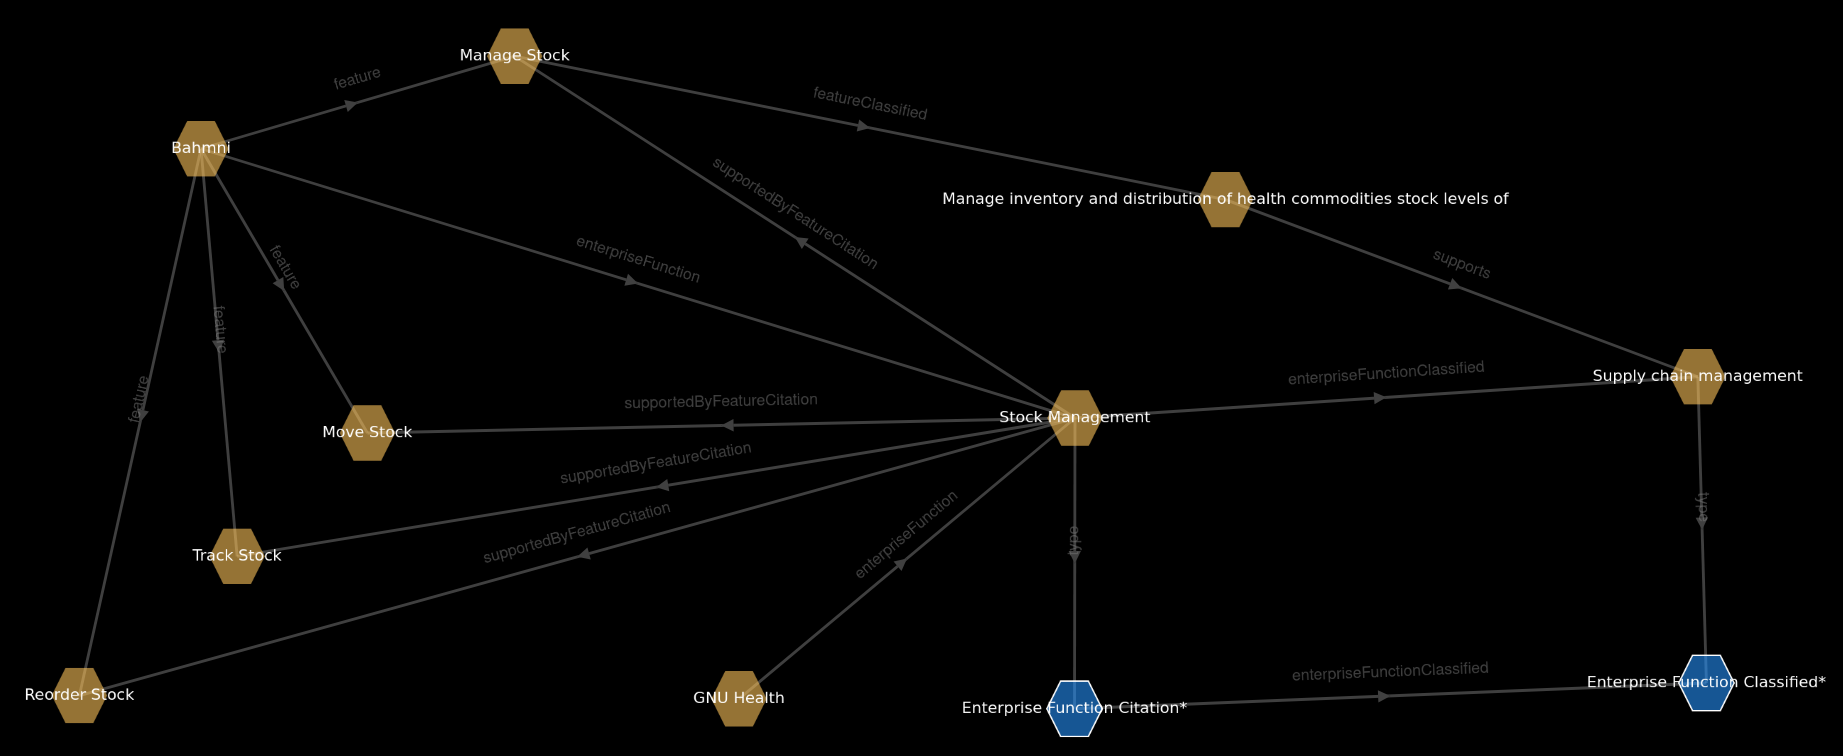
\includegraphics[width=\textwidth, height=.65\textheight]{img/bahmni_star.png}
\end{frame}

\begin{frame}{Verbindung zum Katalogeintrag \enquote{Supply Chain Management}}
  \vspace{-0.5cm}
  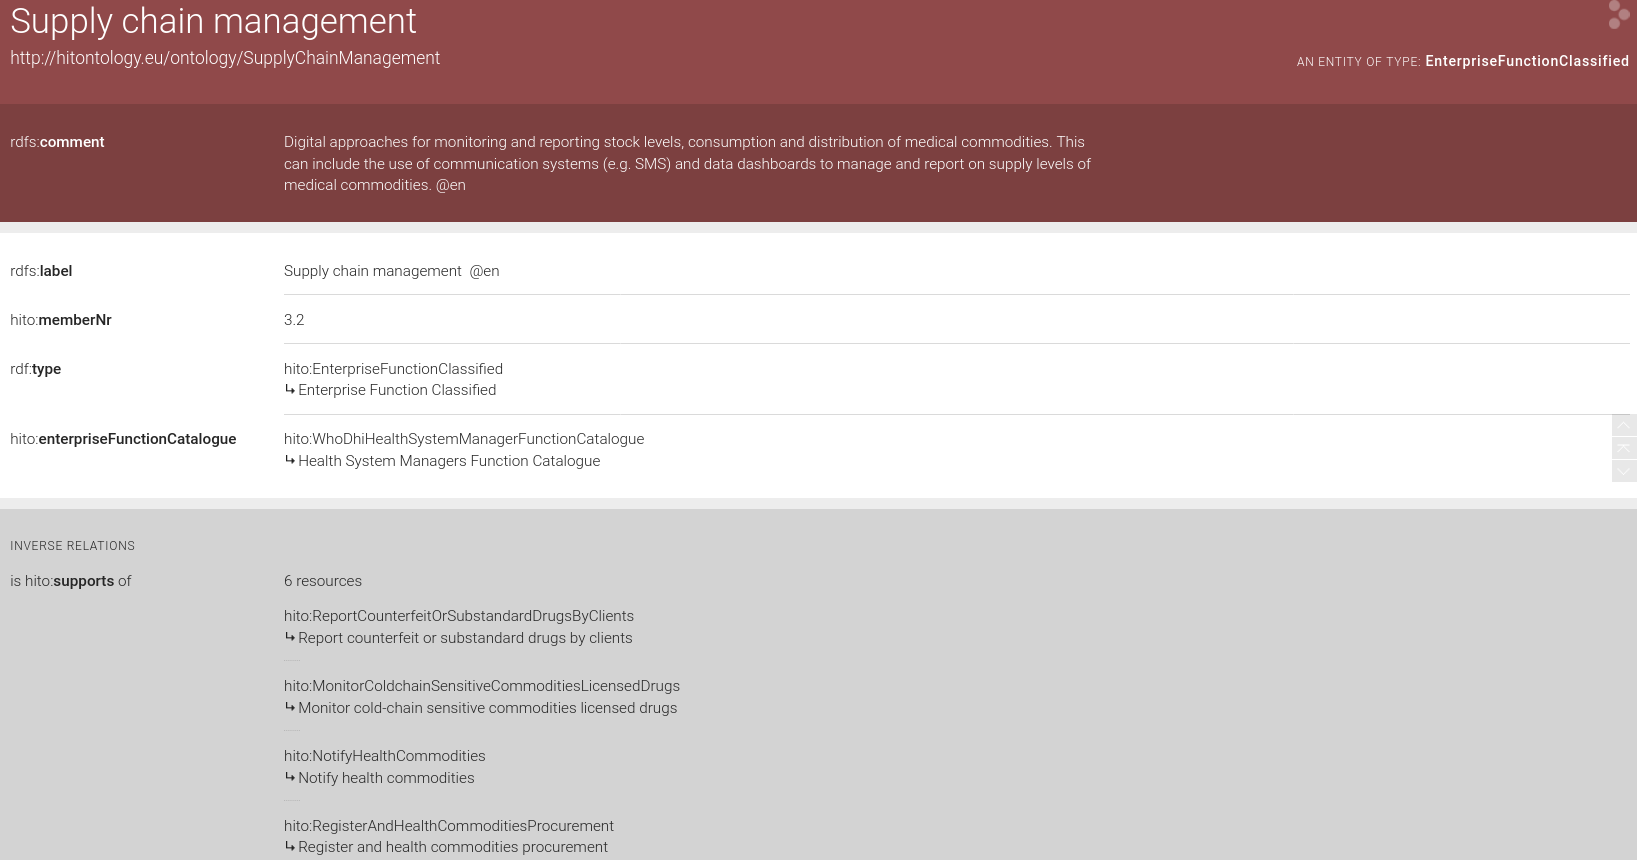
\includegraphics[width=\textwidth]{img/supplychainmanagement.png}
\end{frame}

\begin{frame}{HITO Lifecycle Quality}
  \centering
  \vspace{-0.5cm}
  \cycle{mygreen}{mygreen}{mygreen}{mygreen}{mygreen}{mypink}
\end{frame}

\begin{frame}{Syntaktische Datenqualität -- Ein Beispiel}
  \vspace{-0.3cm}
  \centering
  
\includegraphics[height=.75\textheight]{img/qualitychecker.png}
  \footnotesize{\url{https://hitontology.eu/qualitycheck.html}}
\end{frame}

\begin{frame}{Ausblick}
\begin{spacing}{1.5}
\begin{itemize}
  \item Visualisierung mithilfe anderer Werkzeuge
  \begin{itemize}
    \item Web VOWL
    \item RelFinder
    \item LodLive
  \end{itemize}
\end{itemize}
\end{spacing}
\end{frame}

%\begin{frame}{Ansicht von HITO in WebVOWL}
%  \vspace{-0.3cm}
%  \centering
%  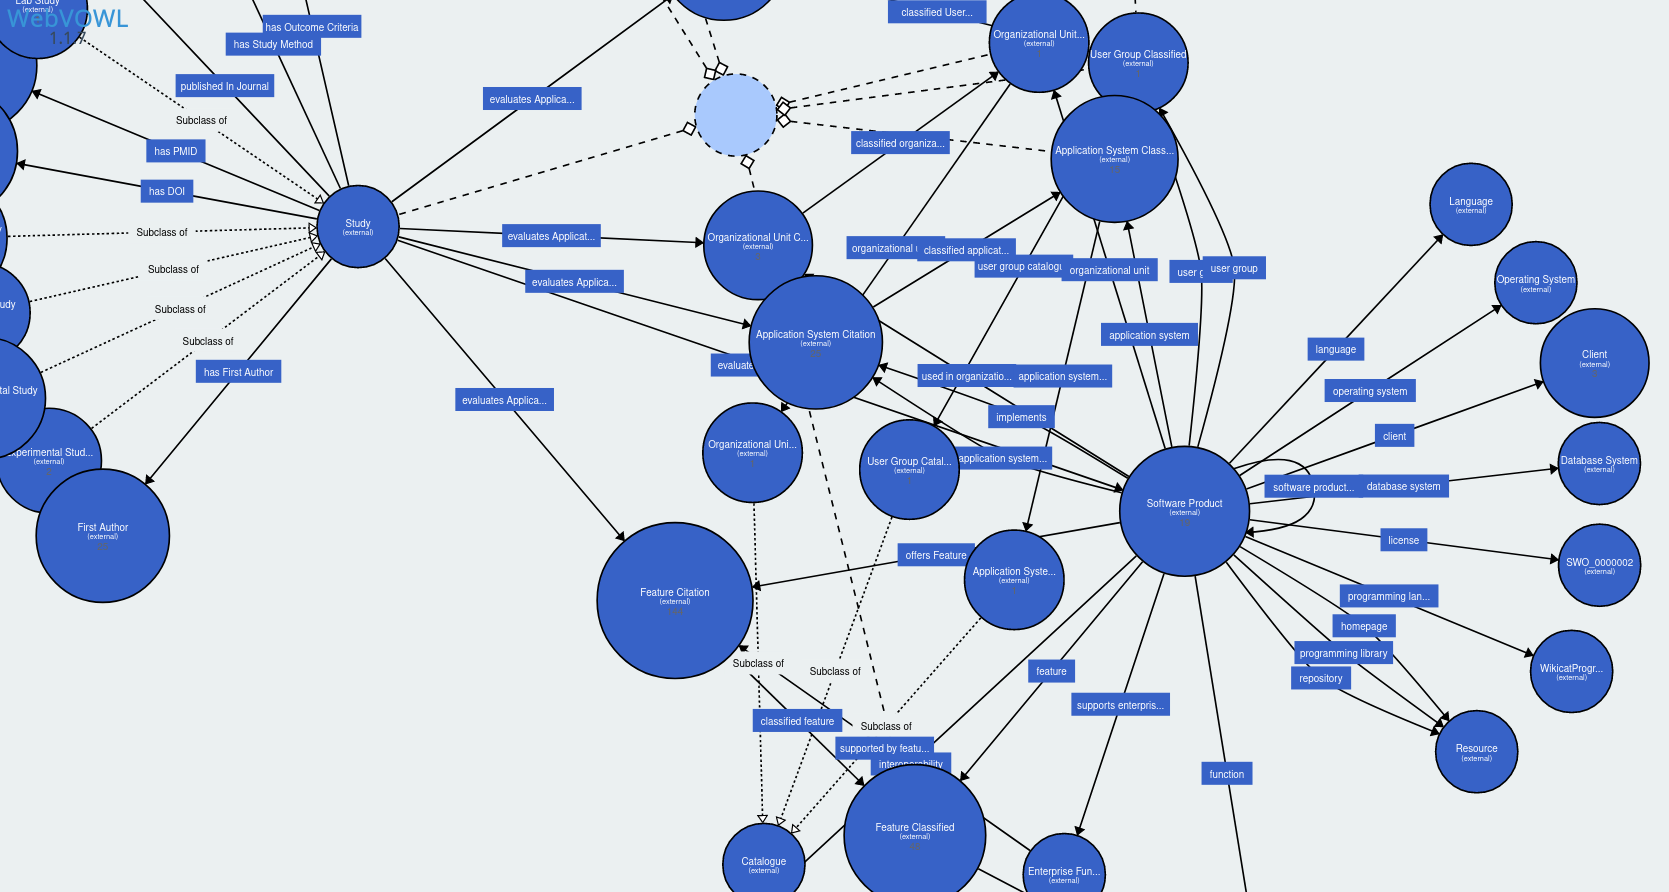
\includegraphics[width=.95\textwidth]{img/webvowl.png}
%  \footnotesize{\url{http://www.visualdataweb.de/webvowl/\#iri=https://raw.githubusercontent.com/hitontology/ontology/master/hito.ttl}}
%\end{frame}

\begin{frame}{Fragen?}
  \centering
  \vspace{-0.5cm}
  
\includegraphics[width=\textwidth]{img/fragen.png}
\end{frame}

\begin{frame}
  \centering
  \huge Szenarien für die Integration von medfloss.org und HITO
\end{frame}

\begin{frame}{Szenario 1: Medfloss.org vollständig ersetzen}
\begin{spacing}{1.25}
\begin{itemize}
\item Nicht möglich für uns
\item Begrenzte Projektlaufzeit, aber unbegrenzte Wartung nötig
\item IMISE: Forschungsprojekte im Vordergrund, Software nur Mittel zum Zweck
\item Keine Alternative zu Community-Werkzeugen für Diskussionen, Ereignisse und Publikationen
\item Datenbank vs. Linked Open Data: siehe Szenario 2
\end{itemize}
\end{spacing}
\end{frame}

\begin{frame}{Szenario 2: Medfloss-Datenbank zu Linked Data konvertieren}
\begin{spacing}{1.25}
\begin{itemize}
\item Datenbankschema zu Ontologie erweitern
\item Datenbankinhalt zu Instanzdaten konvertieren
\item Links zu externen Wissensbasen
\item Synonyme, Homonyme
\item Ressourcen statt Strings
\item $\rightarrow$ manuelle Nacharbeit nötig
\item mehrere in einem Typ: Programming Language vs Library
\end{itemize}
\end{spacing}
\end{frame}

\begin{frame}{Szenario 2: Taxonomie von Medfloss.org}
\centering
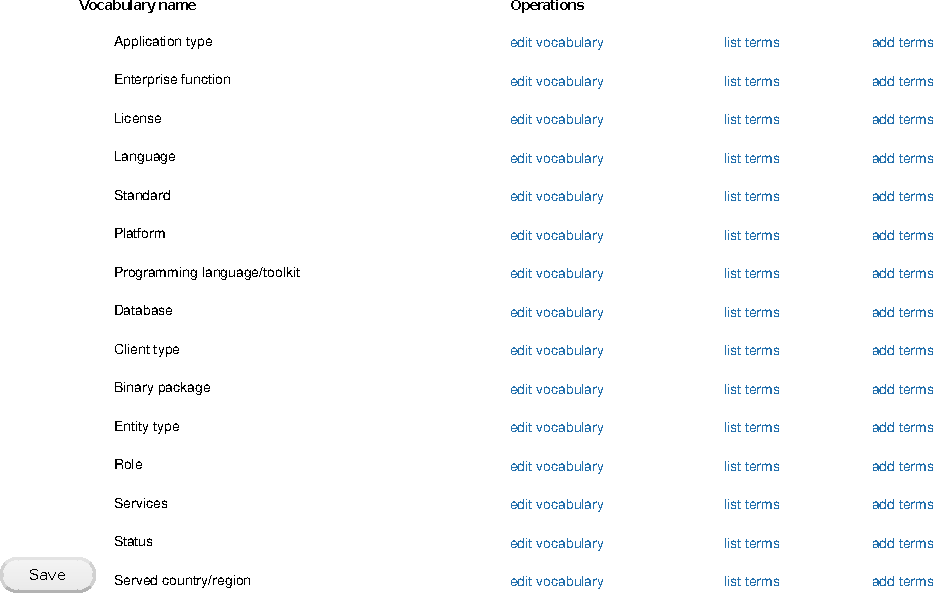
\includegraphics[height=.72\textheight]{img/medfloss-taxonomy.pdf}
\url{https://www.medfloss.org/admin/structure/taxonomy}
\end{frame}

\begin{frame}{Szenario 2: Taxonomie von Medfloss.org -- Enterprise Function}
\centering
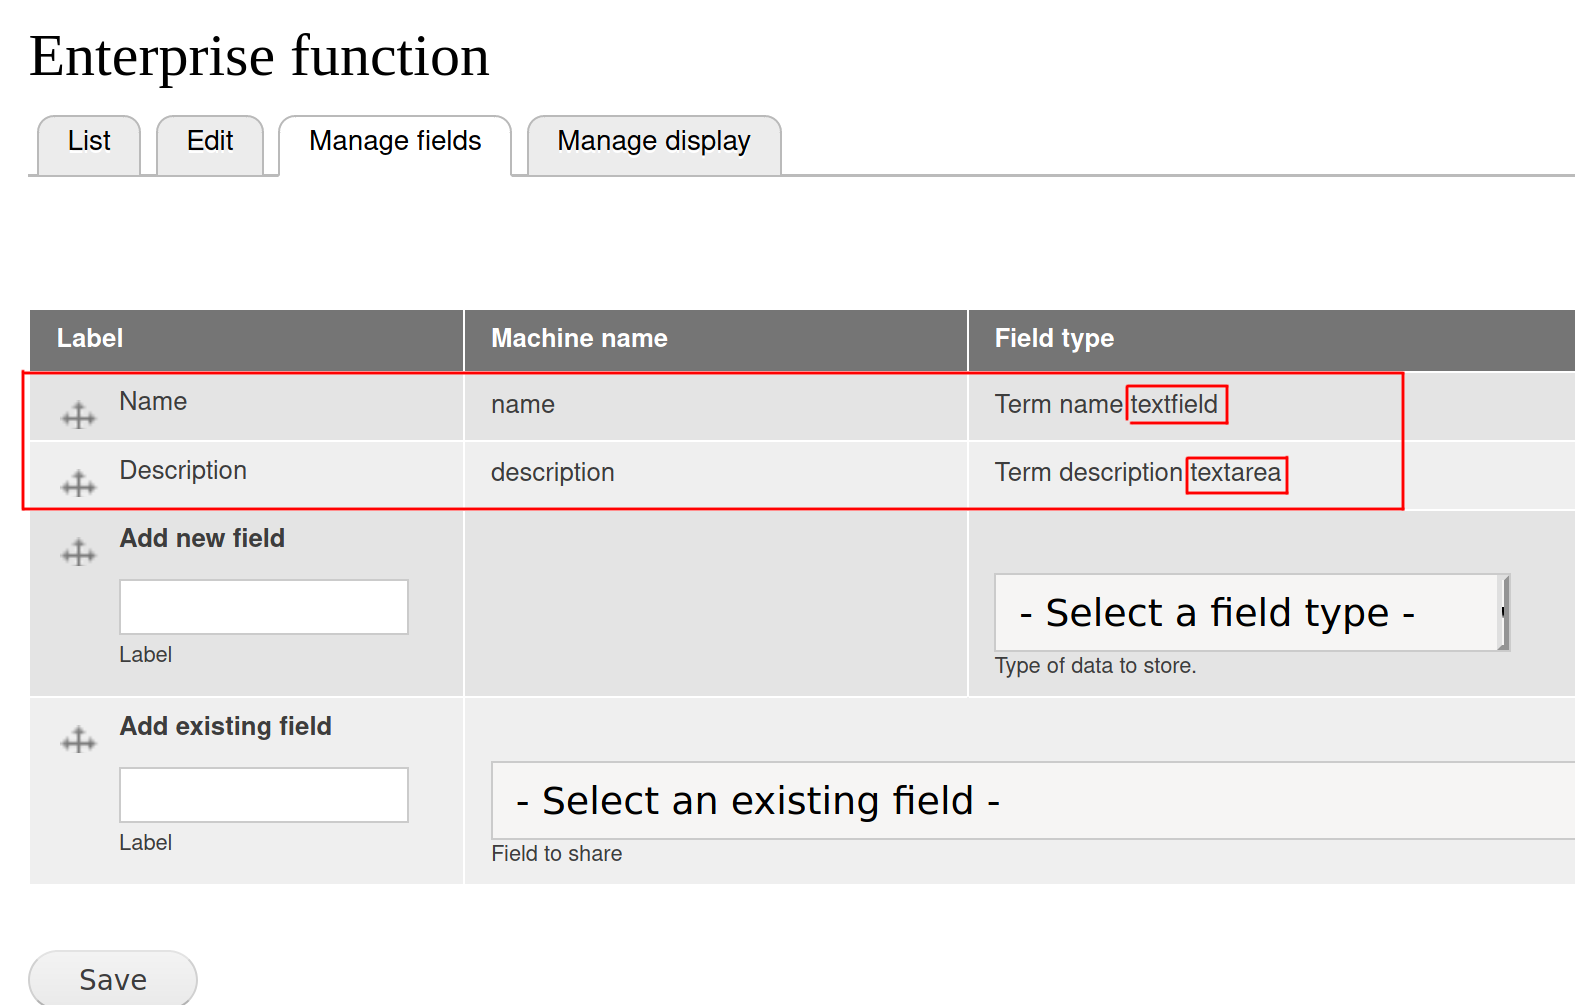
\includegraphics[height=.72\textheight]{img/medfloss-function.png}
\url{https://www.medfloss.org/admin/structure/taxonomy/vocabulary_2}
\end{frame}

\begin{frame}{Szenario 2: Ontologie von HITO -- Enterprise Function}
\centering
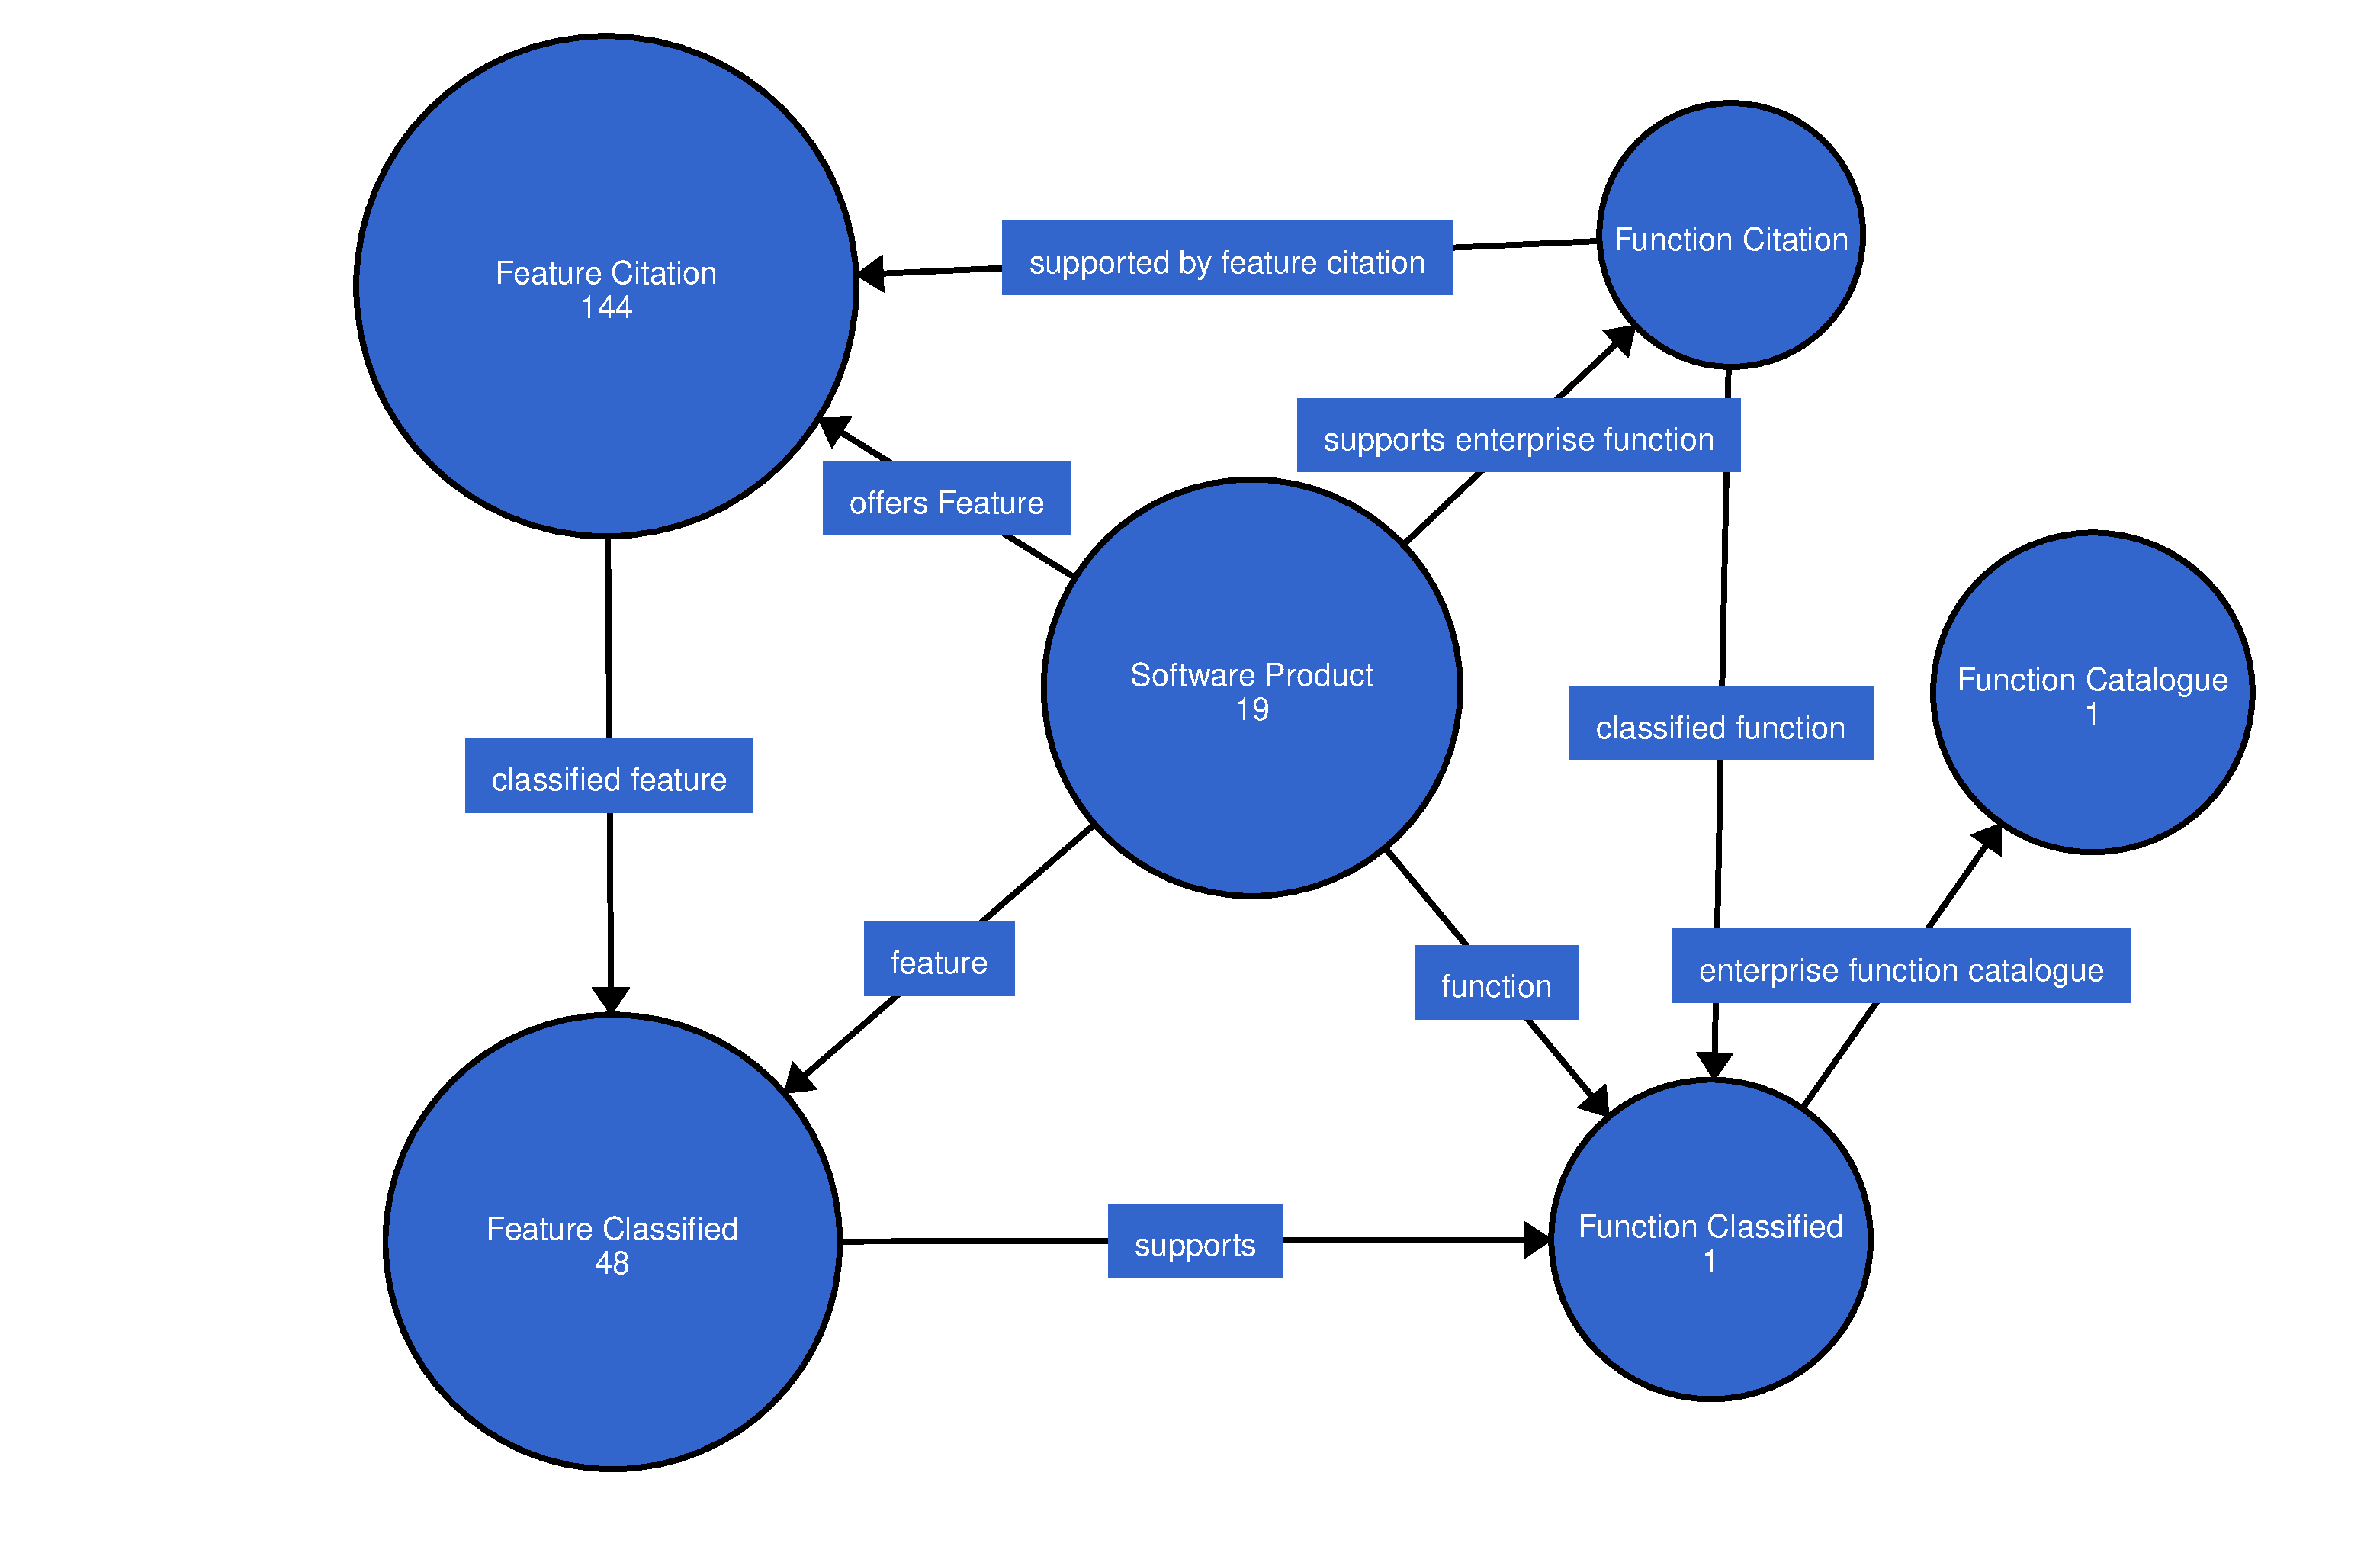
\includegraphics[height=.8\textheight]{img/function.pdf}
\end{frame}


\begin{frame}{Szenario 3: Links zwischen Medfloss und HITO}
\begin{spacing}{1.5}
\begin{itemize}
\item HITO bildet ausgewählten Teil der Medflossprodukte ab
\item dafür mehr Struktur, Qualität und Details
\item Link von jedem Produkt in LodView zu HITO
\item Link von jedem Produkt in Medfloss zu HITO, falls letzteres existiert
\end{itemize}
\end{spacing}
\end{frame}

\begin{frame}{HITO Bahmni}
  \vspace{-0.5cm}
  \centering
  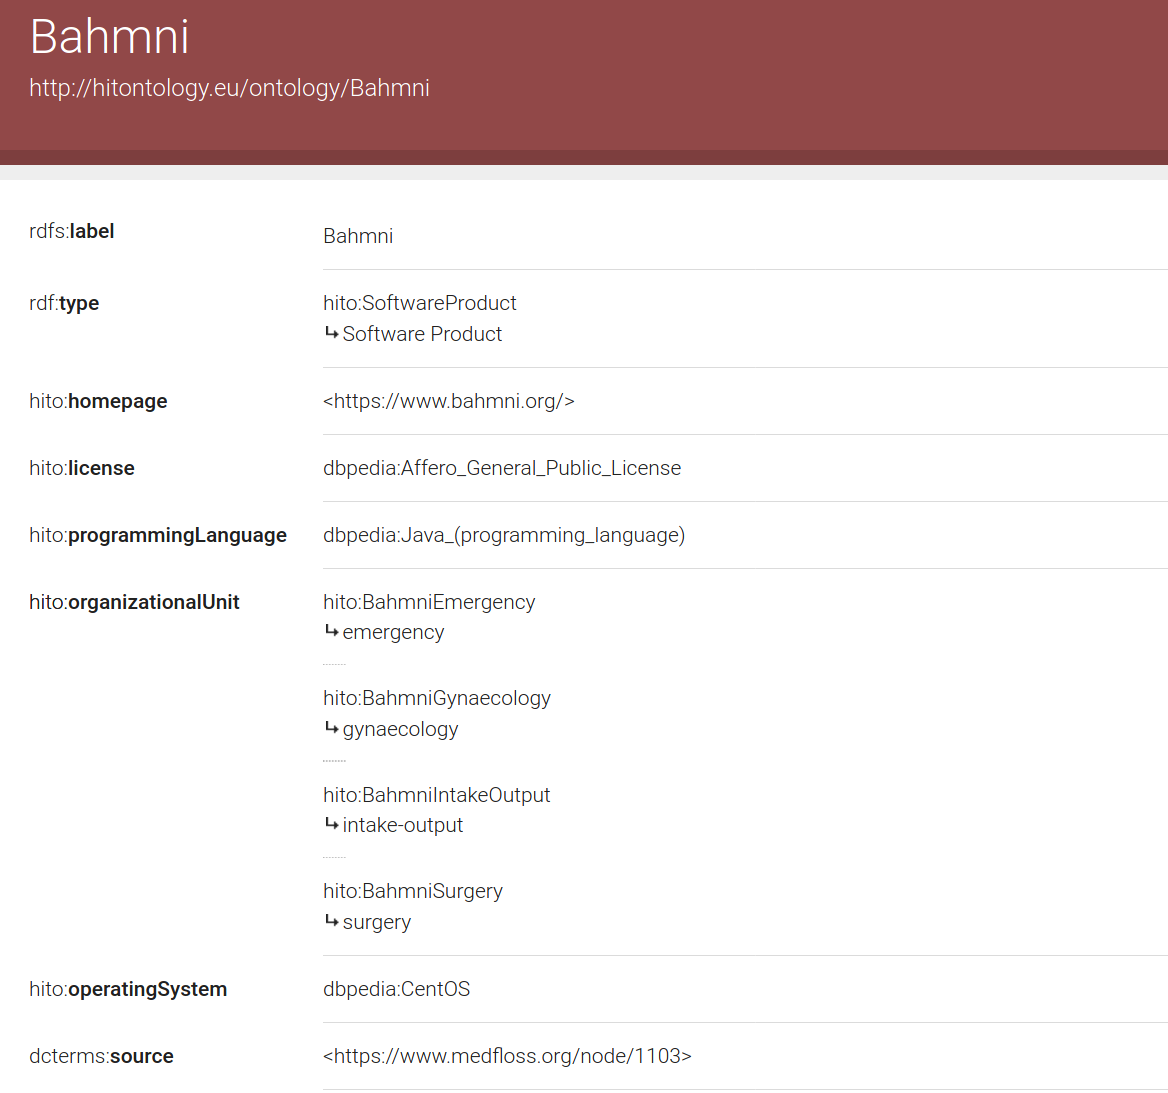
\includegraphics[height=.8\textheight]{img/hito-bahmni.png}
\end{frame}

\begin{frame}{Medfloss Bahmni}
  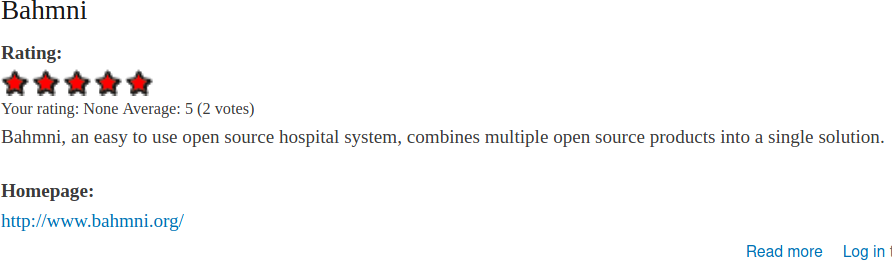
\includegraphics[width=\textwidth]{img/medfloss-bahmni.png}
\end{frame}

\begin{frame}{Medfloss Bahmni Link}
  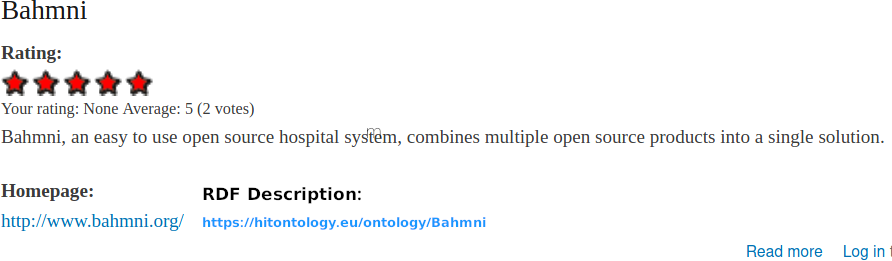
\includegraphics[width=\textwidth]{img/medfloss-bahmni-link.png}
\end{frame}

\begin{frame}{Diskussion}
  \centering
  \vspace{-0.5cm}
  
\includegraphics[width=\textwidth]{img/discussion.png}
\end{frame}

\end{document}
